\documentclass[mscthesis]{usiinfthesis}
\usepackage{lipsum}

\usepackage[linesnumbered,nosemicolon,noline]{algorithm2e}
\usepackage{algpseudocode}
\usepackage{environ}

%For substeps in algo environment
\newcounter{parentAlgoLine}
\SetKwBlock{BEGIN}{}{}

\makeatletter
\NewEnviron{substeps}{%
  \refstepcounter{AlgoLine}% <---- remove if necessary
  \protected@edef\theparentequation{\theequation}%
  \setcounter{parentAlgoLine}{\value{AlgoLine}}%
  \setcounter{AlgoLine}{0}%
  \def\theAlgoLine{\theparentAlgoLine.\arabic{AlgoLine}}%
  \BEGIN{\BODY}%
  \setcounter{AlgoLine}{\value{parentAlgoLine}}%
  \ignorespacesafterend
}
\makeatother

%For algo sub-state

\newcounter{algsubstate}
\renewcommand{\thealgsubstate}{\alph{algsubstate}}
\newenvironment{algsubstates}
  {\setcounter{algsubstate}{0}%
   \renewcommand{\State}{%
     \stepcounter{algsubstate}%
     \Statex {\footnotesize\thealgsubstate:}\space}}
  {}

\usepackage{listings}
\graphicspath{ {./figures/} }

\lstdefinelanguage{algebra}
{morekeywords={import,sort,constructors,observers,transformers,axioms,if,
else,end},
sensitive=false,
morecomment=[l]{//s},
}

% Variables
%\newcommand\numberevents{61751 } % whole dataset
%\newcommand\numberevents{36013 } % number of invasions from 1850 to 2010
%\newcommand\numbereventsfilter{10840 } % number of invasions from 1850 to 2010

% For equations float
\usepackage{float}
\usepackage{aliascnt}
\newaliascnt{eqfloat}{equation}
\newfloat{eqfloat}{h}{eqflts}
\floatname{eqfloat}{Equation}

\newcommand*{\ORGeqfloat}{}
\let\ORGeqfloat\eqfloat
\def\eqfloat{%
  \let\ORIGINALcaption\caption
  \def\caption{%
    \addtocounter{equation}{-1}%
    \ORIGINALcaption
  }%
  \ORGeqfloat
}


\title{Alien species modelling via relational event models} %compulsory
%\specialization{Dependable Distributed Systems}%optional
%\subtitle{Subtitle: Reinventing the World} %optional 
\author{Niccol\`o Zuppichini} %compulsory
\begin{committee}
\advisor{Prof.}{Ernst-Jan Camiel}{Wit} %compulsory
\coadvisor{}{Igor}{Artico}{} %optional
\end{committee}
\Day{23} %compulsory
\Month{June} %compulsory
\Year{2022} %compulsory, put only the year
\place{Lugano} %compulsory

%\dedication{To my beloved} %optional
%\openepigraph{Hello there \dots}{General Kenobi} %optional

%\makeindex %optional, also comment out \theindex at the end

\begin{document}

\maketitle %generates the titlepage, this is FIXED
% this might causes problem...why?
\frontmatter %generates the frontmatter, this is FIXED

\begin{abstract}
\newcommand\numberevents{36013 } % number of invasions from 1850 to 2010

% Topic introduction
During the last centuries, human research on the interaction of species substantially intensified. However, we know little to nothing about the underlying process that shapes the behaviors of alien species invasion across regions, countries, and ecosystems. An alien species is a species found outside of its native region.

% What we do here
In this thesis, we present a novel relational event model approach with an underlying latent space framework. We show how this model can be applied to a bipartite unidirectional graph by studying the real-world case of alien species co-invasion. We fit our model to the most exhaustive dataset of first alien species records currently available.

%% What we got
Using years of first records of 36013 invasions of alien species from 18 taxonomic groups spanning from 1850 to 2010 we show how a custom relational event model can be used to model the dynamics of species co-invasion by embedding the species-region interactions into a latent space. We then show how to infer the structure of this space and the relationship between species and regions. 

%Furthermore, due to the high size of the dataset, we also present a high-performance python implementation of our model.

The goal of this thesis is twofold: to show a novel approach to REM by using an underlying latent space and to show a real-world application of the model.

%TODO briefly report results

\end{abstract}

%\begin{acknowledgements}
%\lipsum 
%\end{acknowledgements}

%\tableofcontents 
%\listoffigures %optional
%\listoftables %optional

\mainmatter

\chapter{Introduction}
% 1. Motivation. Why invasive species are a problem?
% 2. Briefly introduce the dataset
% 3. Briefly introduce how I will study the dataset
% 4. Briefly introduce how I will study the dataset
% 5. TODO briefly report the results

%Introduce problem
The rate at which alien species invade countries have increased over the last century and it is becoming an important issue. The economic impact of alien species in Europe is estimated to be close to 13 billion dollars annually \cite{intro:rate}. The interest in the study of the dynamics of alien species has been increasing over the years for this reason. Unfortunately, due to the complexity of the problem, is hard to come up with real actions. Intuitively, the invasion rate of species differs belonging to different taxonomic groups, however, a comprehensive global invasion dynamics study of the last centuries subdivided by taxonomic groups is still lacking. The dynamics of invasive species are driven by a multitude of factors simultaneously. These factors can be complex involving exogenous, endogenous, sociological, ecological, and socio-economic factors \cite{intro:factors}. It is important to develop a framework capable of studying and analyzing all these underlying effects simultaneously. 

%Describe approach
A relational event is an interaction between a sender and a receiver at a specific timestamp. An invasion of a species into a region can be described as a relational event. A relational event model (REM) studies the temporal sequence of such relational events. REM was first developed in the field of social network analysis \cite{rem:butts}. This framework has many advantages in the fact that it is able to study underlying temporal patterns, can efficiently deal with time-varying variables and it is an extremely adaptable hypothesis testing tool. Due to its versatility, in the years it is been applied in a large number of different fields such as animal-animal interaction \cite{intro:cattle}, the evolution of team networks \cite{intro:teams} and national hospitals collaborations in transfering critical patients \cite{intro:hospital}. 

%What has been already done and what is the problem
In the years, there have been a large number of different statistical approaches with the goal of predicting and describing the spread of alien species. However, traditional statistical tools, such as multidimensional scaling, fail to capture the similarity of nodes on this kind of dataset due to their bipartite nature (i.e. no interaction of the kind species-species and region-region). A REM approach is a good approach to this problem, however, due to the high number of possible local network configurations, it is really hard to keep track of the past configurations to study dynamic networks.

%TODO add a citation on this REM

%Our approach and how it is better

In this thesis, we contribute to the practical applicability of a REM with a latent space underlying framework modeled on a bipartite social network graph with a real-world case study of the dynamics of co-invasion of species. Our model is capable of taking multiple species simultaneously into consideration and to study the underlying relationship between different species co-invading regions by training on the most exhaustive source of first records of alien species in multiple regions in the world. We propose a different approach from the traditional literature by disposing the species and regions (which sometimes I simply refer to as nodes) into a latent space and by fitting a custom REM on it. By studying the proximity of the nodes in the latent space, our model is capable of determining the group of nodes that tend to co-invade a region and, in an analogous way, the group of regions that are more likely to be invaded by the same group of species.  By disposing of the species-region interactions in a latent space we "summarise" their configuration history hence we can effectively approximate the past information and train a REM more efficiently. In this space, nodes are allowed to move by attracting or repulsing other nodes. The closeness between nodes describes they tend to interact (which is to co-invade a region). Within the limits of this latent space configuration, a node location at a certain time describes his history evolution and by studying this evolution we can infer the group of nodes that have similar tendencies and behaviors.


% Structure of the thesis
We structure the rest of this thesis as follows. In chapter 2 we make a preliminary study of the dataset of the alien species and discuss previous research. In chapter 3 we present an exhaustive statistical background of the methods used for the reader. In chapter 4 we provide a formulation of our latent space REM and show how to make inferences on it. In chapter 5 we report our results. In the conclusive chapter 6, we conclude with a final discussion.


%TODO briefly report the results(?)

\chapter{Materials and methods}
\label{sec:dataset}
Our study of the co-invasion of species is based on the Alien Species First Records database \cite{intro:dataset} which to date is the most exhaustive source of first records of alien species currently available. The dataset contains the years of the first establishment of alien species in regions worldwide. This dataset has been updated many times to include a more in-depth amount of data on the alien species \cite{intro:datasetv2} and nowadays still in continuously update. The current version includes 61751 invasions of 23191 species divided into 18 taxonomic families (listed in Tab. \ref{table:families}) in 276 regions\footnote{Regions generally correspond to countries but in the dataset available almost half regions are islands.} ranging from 7000 AD to 2020.


\begin{table}[H]
\centering
\begin{tabular}{|l|l|l|l|l|}
\hline
Algae      & Birds       & Fishes        & Mammals  & Vascular plants \\ \hline
Amphibians & Bryophytes  & Fungi         & Molluscs & Viruses         \\ \hline
Arthropods & Bryozoa     & Insects       & Reptiles &                 \\ \hline
Bacteria   & Crustaceans & Invertebrates & Spiders  &                 \\ \hline             
\end{tabular}
\caption{The 18 taxonomic families.}
\label{table:families}
\end{table}

We focus our research on the time interval spanning from 1850 to 2010. Taking into consideration all taxonomic families, this timeframes covers a total of 19390 alien species. As Fig. \ref{fig:hist_tax_fam} shows, the distribution of alien species is not uniform between taxonomic families, with the largest two taxonomic families in the dataset being the "Vascular Plants" and "Insects". This is important to take into consideration when analyzing the results because a non-uniform distribution of species into taxonomic families will result in a higher probability of a species interacting, in some way, with a species belonging to one of the most abundant taxonomic families.
%Info right after import t = (1850, 2010)
%There are 18 families and 276 regions
%There are 19390 species.

\begin{figure}[H]
\centering
\begin{minipage}{.55\textwidth}
    \centering
    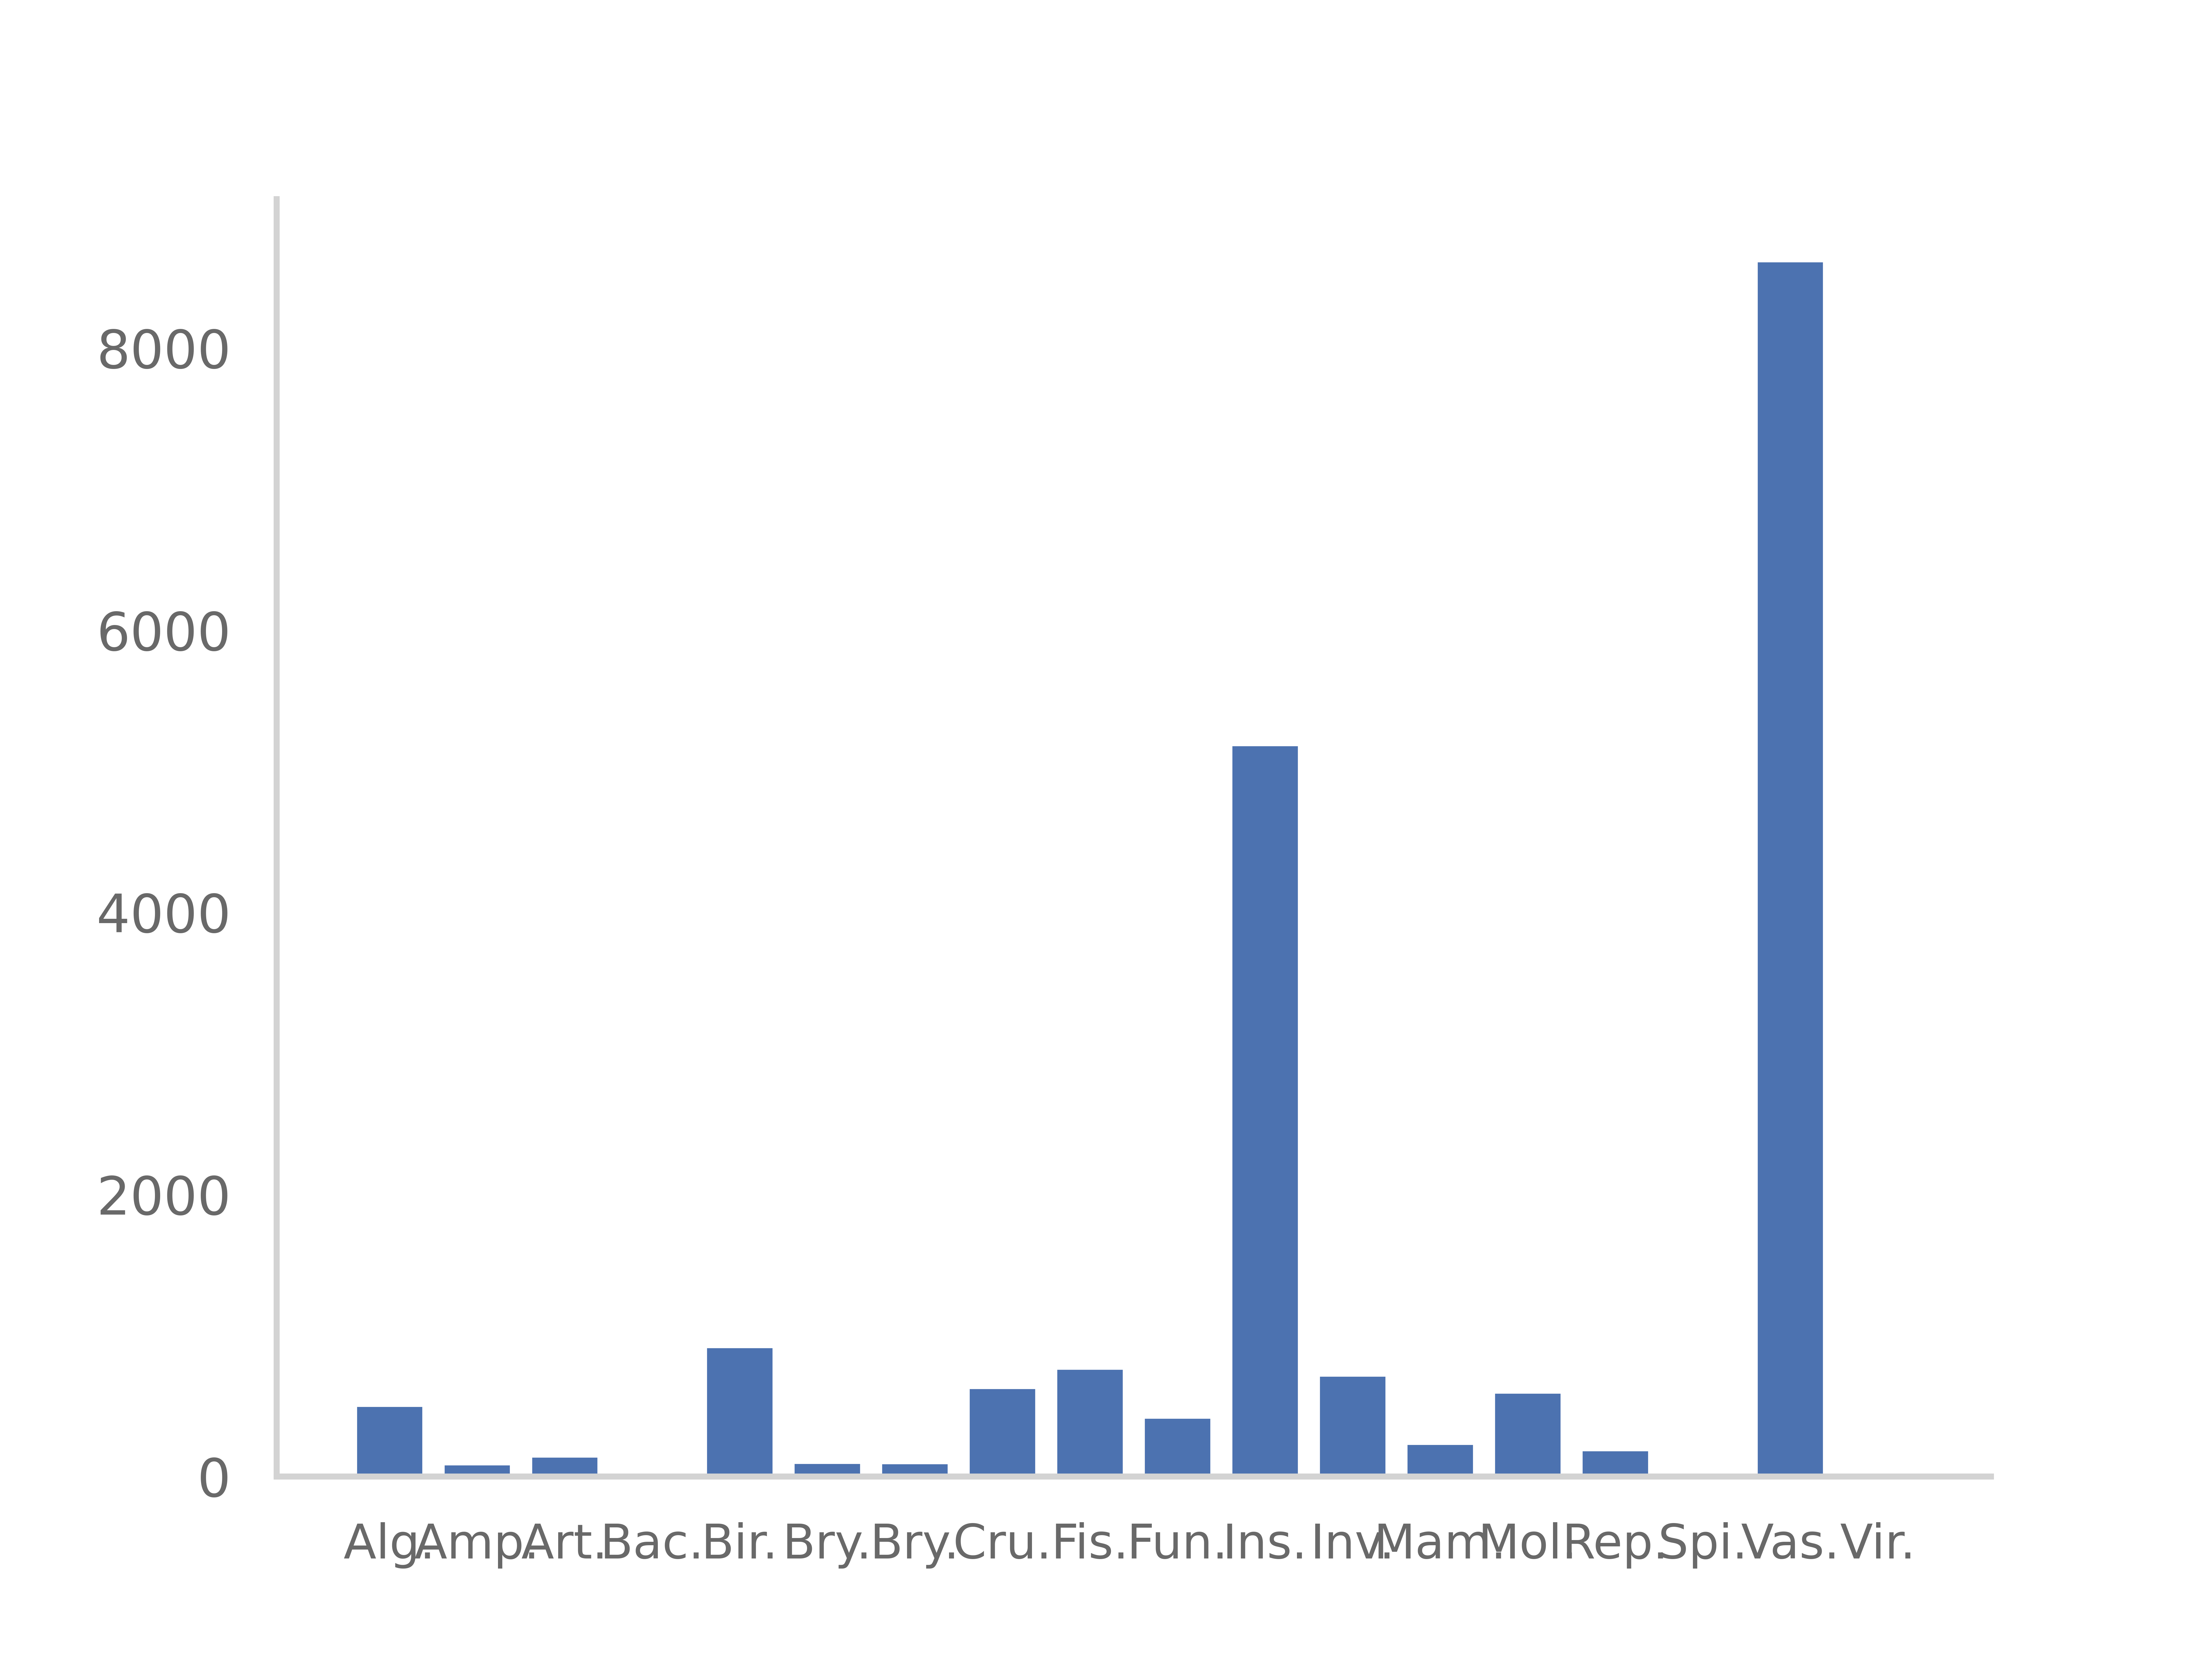
\includegraphics[width=0.9\textwidth]{histogram_taxfam}
    \caption{Histogram of Taxonomic Families \\ and their respective number of alien species in the interval from 1850 to 2010.}
    \label{fig:hist_tax_fam}
\end{minipage}%
\begin{minipage}{.55\textwidth}
    \centering
    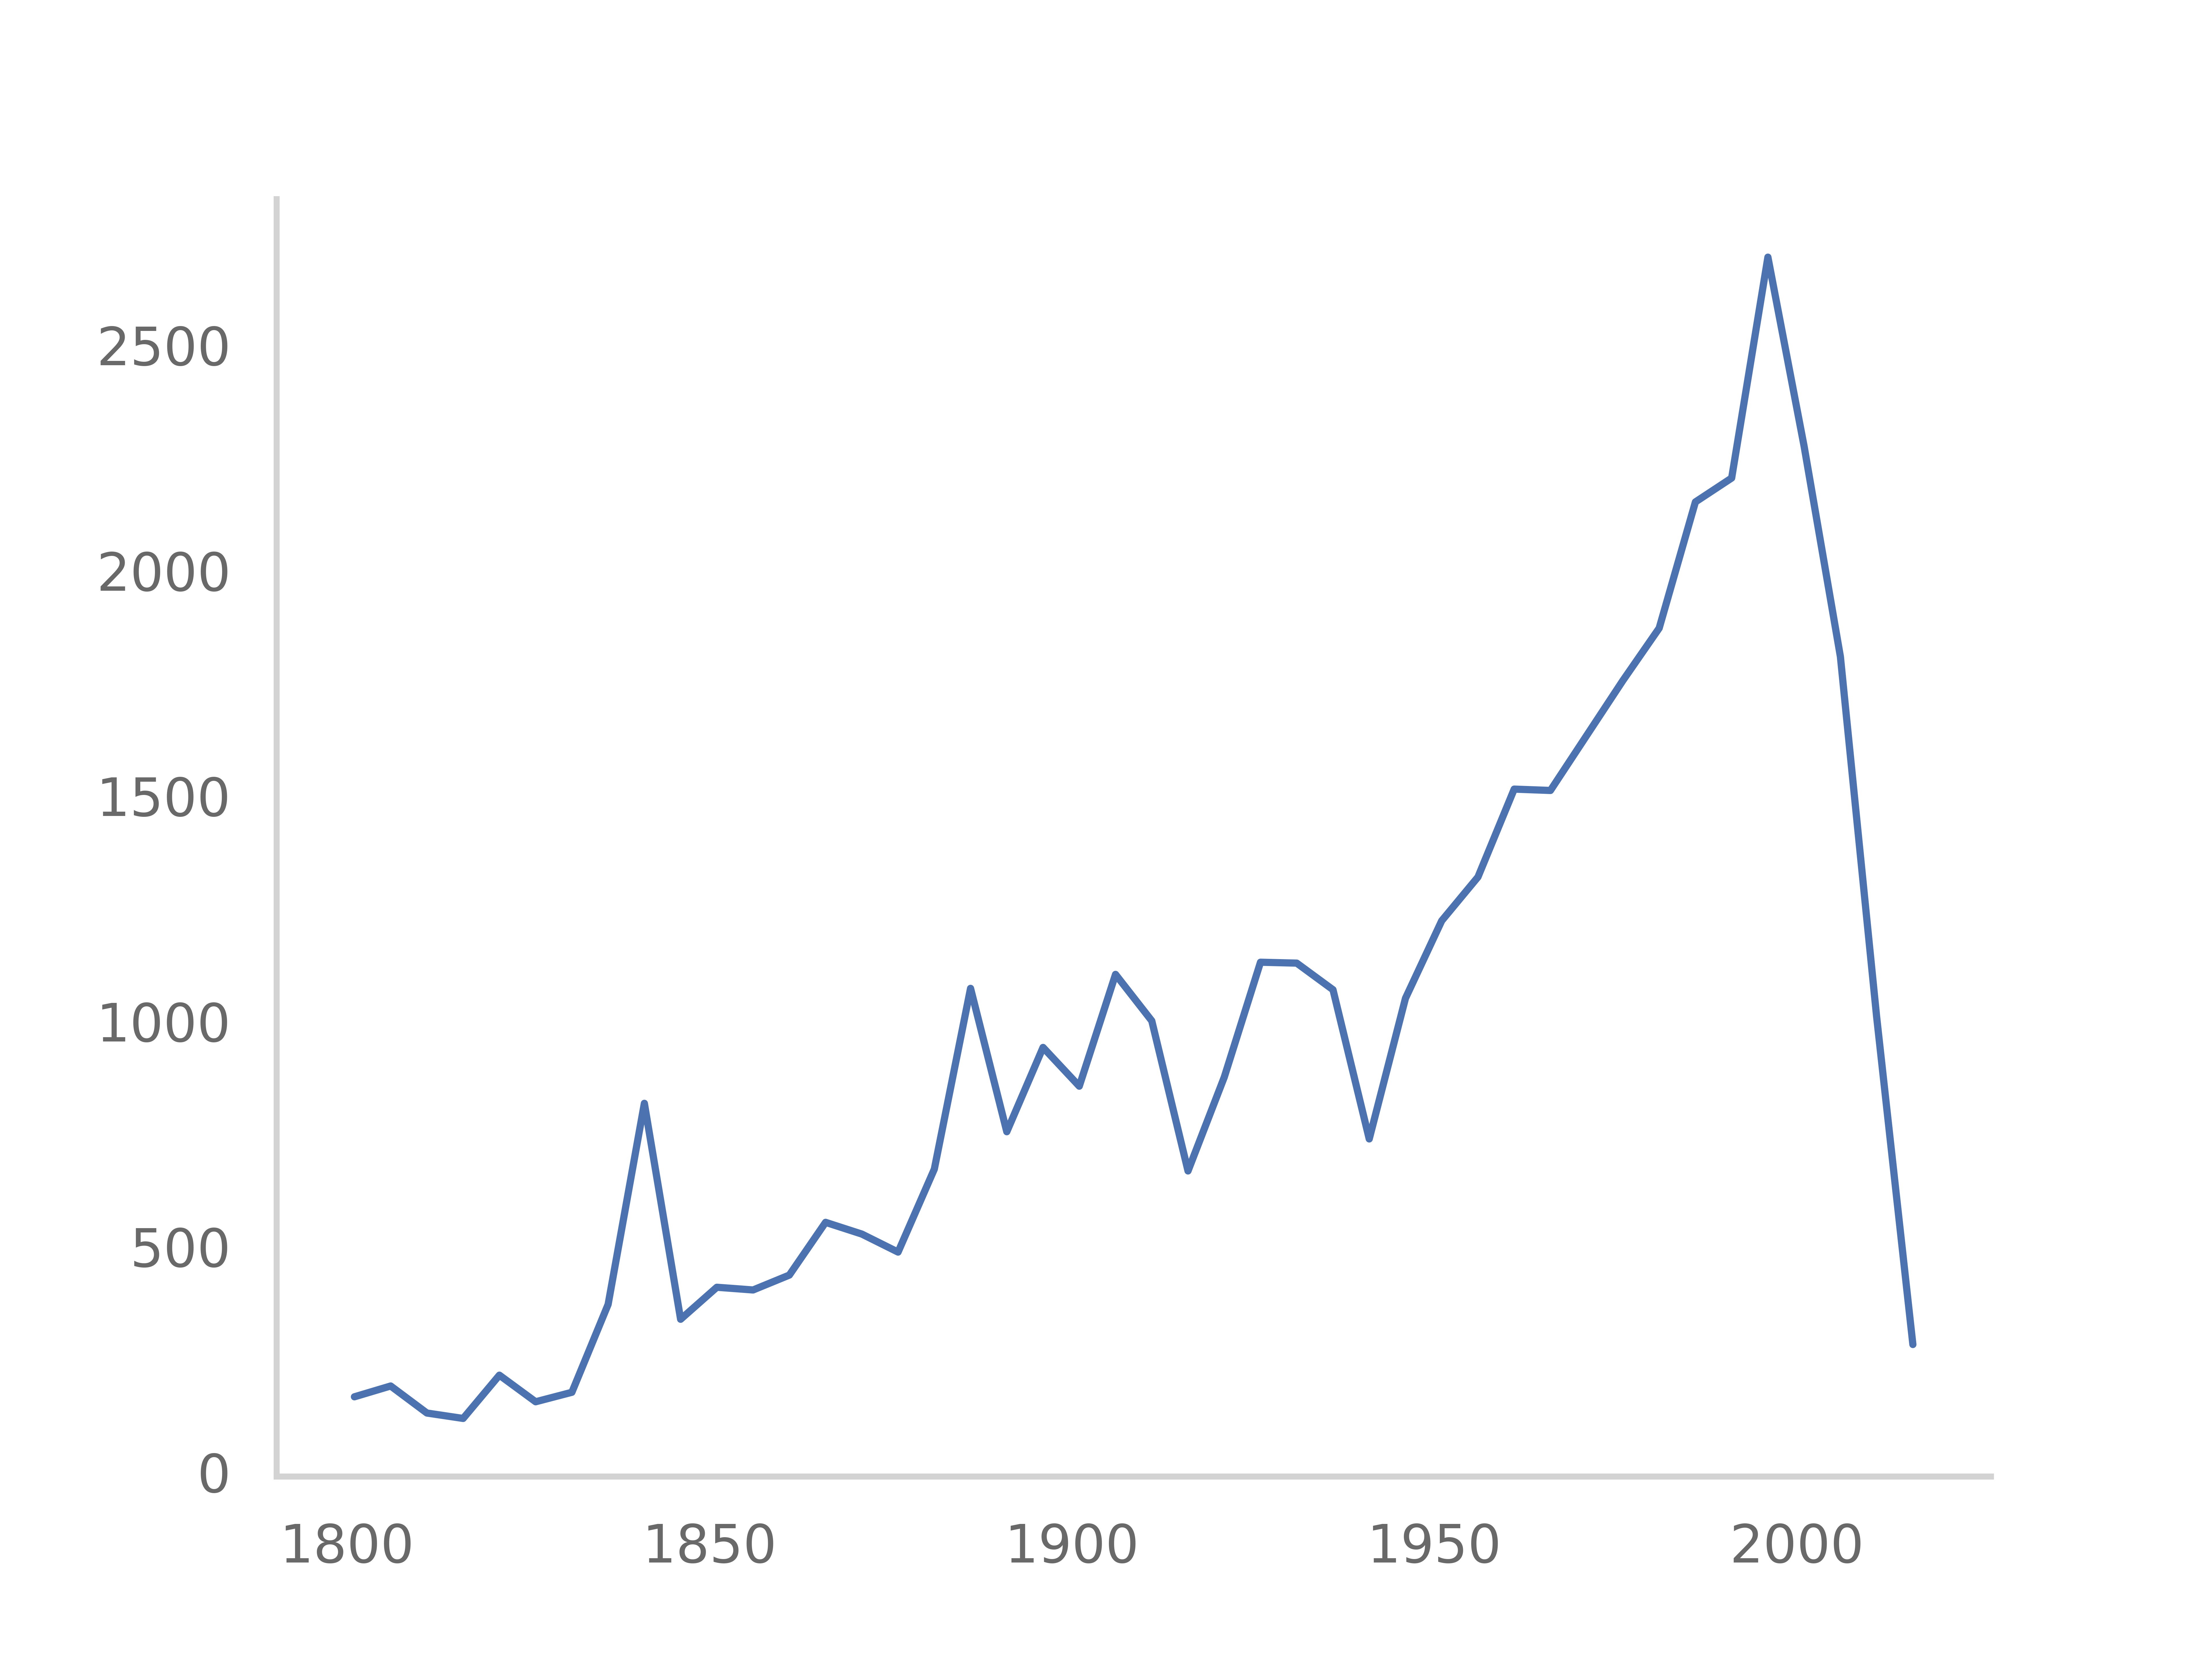
\includegraphics[width=0.9\textwidth]{invasion_per_year.png}
    \caption{Number of invasion per year from 1800 to 2020.}
    \label{fig:invasion_per_year}
\end{minipage}
\end{figure}

Intuitively, the amount of invasion per year increases over time mainly due to factors such as worldwide effects such as the growth of intercontinental trading and an increased worldwide connectivity \cite{intro:ecological}. This claim is indeed supported by the dataset. The number of invasions per year is monotonically increasing (Fig. \ref{fig:invasion_per_year}). The high downward trend around the year 2000 of invasions should not be trusted because the dataset is being constantly updated and most recent data may still be missing. With the same argument, data before 1850 may not be accurate and reliable enough for an in-depth study. For these reasons, we decided to trim the dataset from 1850 to 2010 to ensure the trustiness of the data. 

% ------- ten most invaded regions ---------
%\begin{table}[ht]
%\centering
%\begin{tabular}{|l|l|}
%\hline
%australia      & 4625 \\ \hline
%belgium        & 2627 \\ \hline
%united kingdom & 2627 \\ \hline
%norway         & 2602 \\ \hline
%united states  & 2420 \\ \hline
%new zealand    & 1498 \\ \hline
%czech republic & 1437 \\ \hline
%austria        & 1333 \\ \hline
%germany        & 1306 \\ \hline
%sweden         & 1211 \\ \hline
%\end{tabular}
%\caption{The 10 most invaded region.}
%%\end{table}
% -----------------------------------------

\begin{figure}[H]
    \centering
    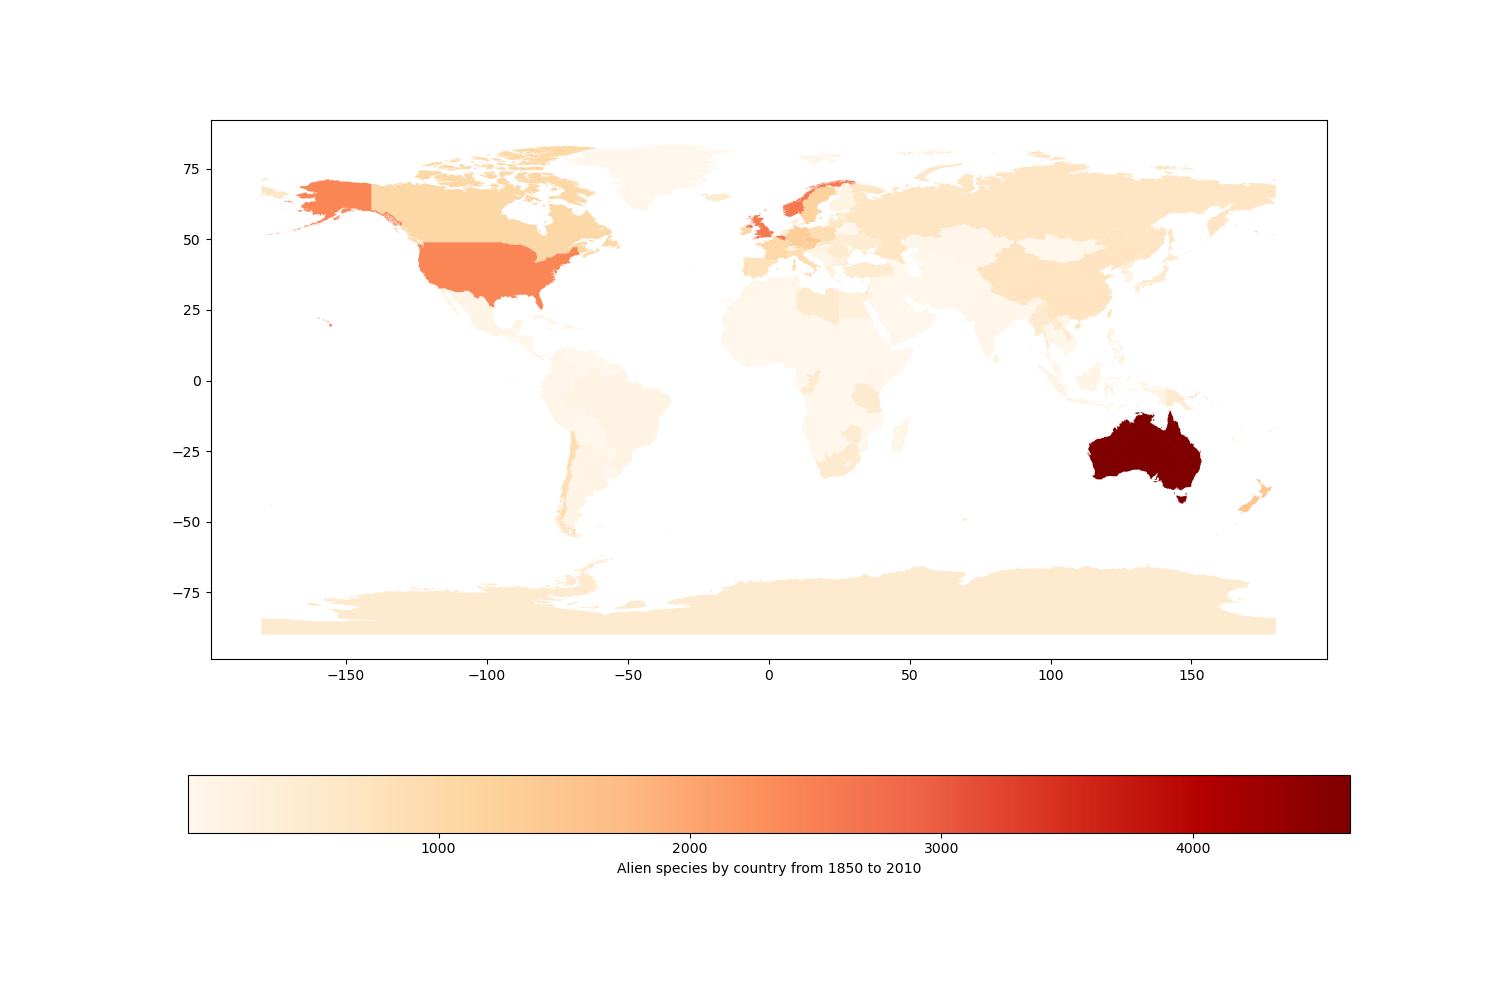
\includegraphics[width=0.85\textwidth]{region_invasion.png}
%    \caption{Symmetric interactions between insects in co-invading events. Each node represents a species and the edge represents the strength of the co-invasion factor. A thick edge indicates that a spread of one of the two species in the relationship is tipically followed by the invasion of the second. Image gently taken from \cite{intro:ecological}}
    \label{fig:region_invasion}
\end{figure}

Contrary to what was expected, some regions have a significantly larger number of invasions during this timeframe. Australia has had more than 4000 invasions. Belgium, the UK, USA, and Norway more than 2000. In contrast, most of the regions in the dataset have less than 3 invasions. Switzerland has been invaded 258 times. Considering that the average number of invasions per region is 200, the distribution of invasion species per region is largely skewed.

% -------------- side by side is ugly as hell ---------------------------------------
%\begin{table}[ht]
%\begin{minipage}[b]{0.2\linewidth}
%\centering
%\begin{tabular}{|l|l|}
%\hline
%Region & Invasions \\ \hline
%australia      & 4625 \\ \hline
%belgium        & 2627 \\ \hline
%united kingdom & 2627 \\ \hline
%norway         & 2602 \\ \hline
%united states  & 2420 \\ \hline
%new zealand    & 1498 \\ \hline
%czech republic & 1437 \\ \hline
%austria        & 1333 \\ \hline
%germany        & 1306 \\ \hline
%sweden         & 1211 \\ \hline
%\end{tabular}
%\caption{The 10 most invaded region.}
%    \label{table:student}
%\end{minipage}\hfill
%\begin{minipage}[b]{0.8\linewidth}
%\centering
%\hfill
%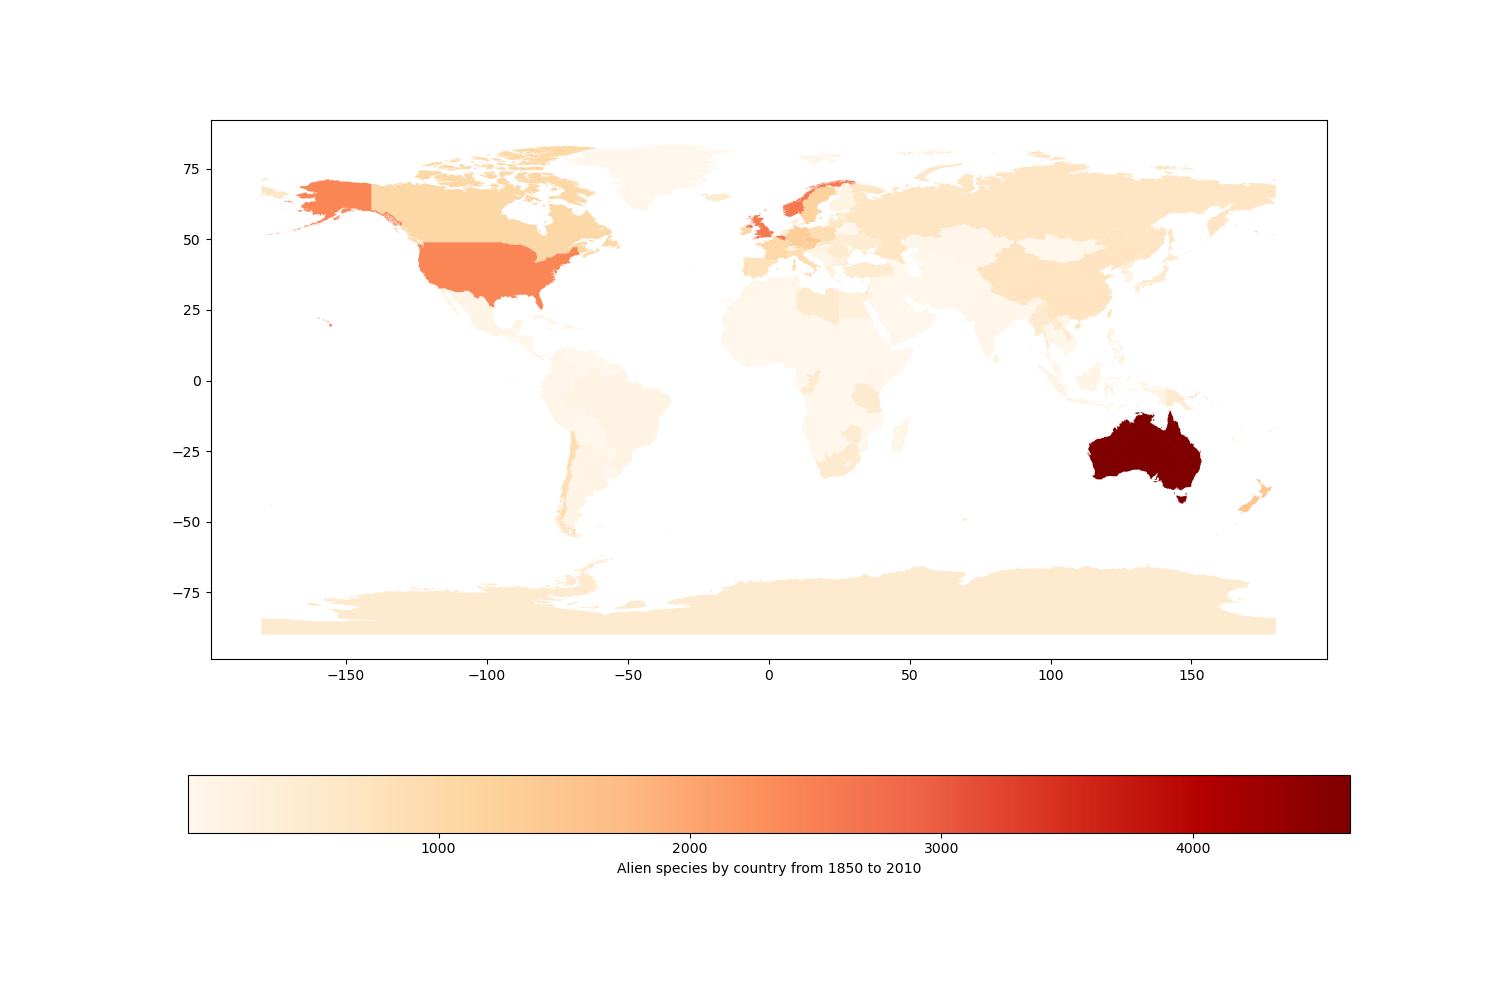
\includegraphics[width=0.85\textwidth]{region_invasion.png}
%%\captionof{figure}{2-D scatterplot of the Student Database}
%\label{fig:image}
%\end{minipage}
%\end{table}
% -------------- side by side is ugly as hell ---------------------------------------

\begin{figure}[H]
    \centering
    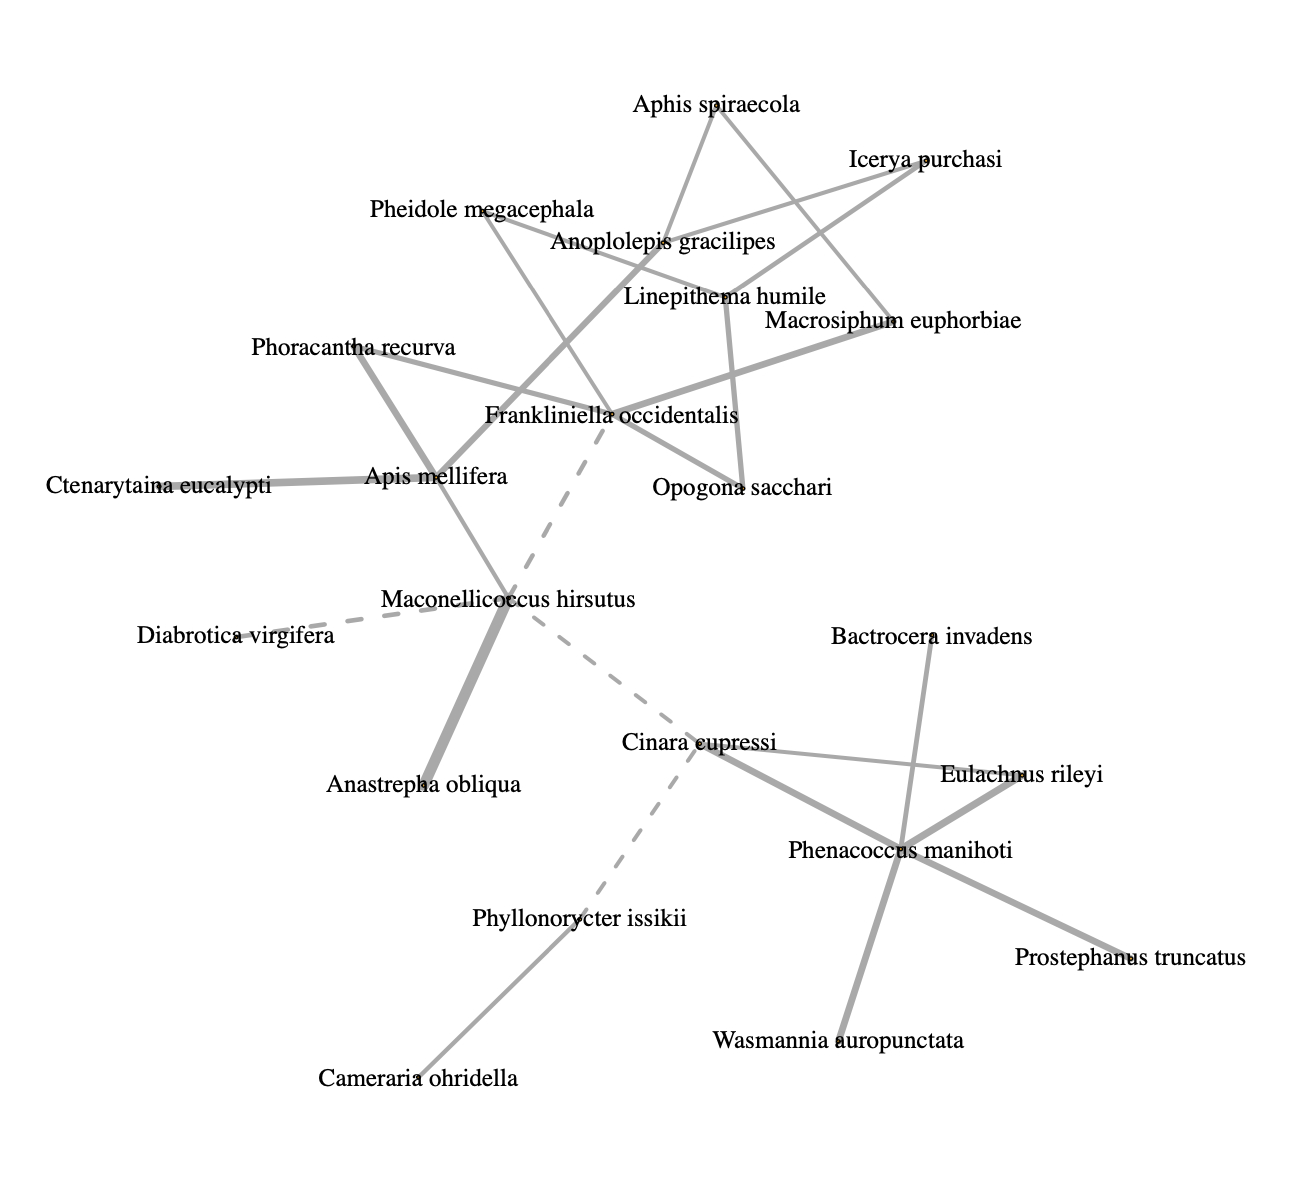
\includegraphics[width=0.75\textwidth]{coinvasion.png}
    \caption{Symmetric interactions between insects in co-invading events. Each node represents a species and the edge represents the strength of the co-invasion factor. A thick edge indicates that a spread of one of the two species in the relationship is tipically followed by the invasion of the second. Image gently taken from \cite{intro:ecological}}
    \label{fig:hist_tax_fam}
\end{figure}

The peak number of invasions per year is close to 5000 invasions around the year 2000, with an average number of invasions per year during the study of about 2800. Considering this number of average invasions per year and the fact that there are more than 20'000 species the dataset is considered to be sparse. To effectively show the high sparsity of the dataset conveniently, I reported two probability density functions (PDF). The PDF shown in Fig. \ref{fig:pdf_invasion} is left-skewed with a mean of 4 and a standard deviation of 5, this means that most species only invaded 4 regions out of the 276 in the entire timeframe of our study. It is worth mentioning that the maximum number of invasions is 97 with one outsider that invaded 176 regions. Due to the high sparsity of the dataset and the large computational cost of our method, we made a couple of assumptions to reduce the data complexity and intrinsic computational requirements. 

The first assumption is that any species that did not invade at least 5 regions during the entire timeframe is not relevant to our study. We hence removed more than 14'000 species resulting in a more computationally manageable dataset of around 1700 species. In Fig \ref{fig:pdf_invasion} I reported the resulting PDF resulted by removing all species that did not invade at least 5 regions. 

The second assumption is that islands do not significantly contribute to the diffusion of species. We hence removed 123 regions from the dataset corresponding to islands. The reason to remove islands is two-fold. First, we are mostly interested in studying the interactions of alien species between larger regions and islands are typically not large enough to be significant. Furthermore, long-distance invasions \footnote{The distance between regions is considered as the distance between the closest borders.} are typically rare \cite{paper:lady} and islands are generally more remote. This assumption is supported by the dataset, the average number of invasions that happened in islands is 80 compared to the 200 average invasions of all regions combined. However, there are a couple of islands worth mentioning that contrast this assumption. The Hawaiian Islands and the Azores islands have more than 1000 invasions. We are interested in studying large region interactions and islands generally are "intermediary steps" in long-distance interactions between large regions such as continents. Removing these intermediary steps does not affect the interaction between larger regions, which we are interested in.

%Species belonging to the same taxonomic family are not expected to have a tendency to co-invade regions.
%TODO what does the lady say about co-invasion?
%We are interested in studying the co-invasion of species. Typically, co-invasion is expected to happen between species belonging to different taxonomic families. 

%TODO not yet decided how much filtering. Also, update the number of islands we removed
%TODO maybe extend the discussion on Hawaiian islands? https://en.wikipedia.org/wiki/Invasive_species_in_Hawaii

%it is also worth mentioning that the effect of distance between regions on the invasion rate has largely grown over time, in fact, the rate of the discovery of alien species has increased with di

Under these two assumptions, we filtered all non-irrelevant species and regions out of the dataset to $1724$ species and $153$ regions and $15947$ invasions from $1850$ to $2010$.

%TODO check these numbers
%%Info right after removing islands
%There are 18 families and 153 regions
%There are 15947 species.

 
\begin{figure}
\centering
\begin{minipage}{.5\textwidth}
  \centering
    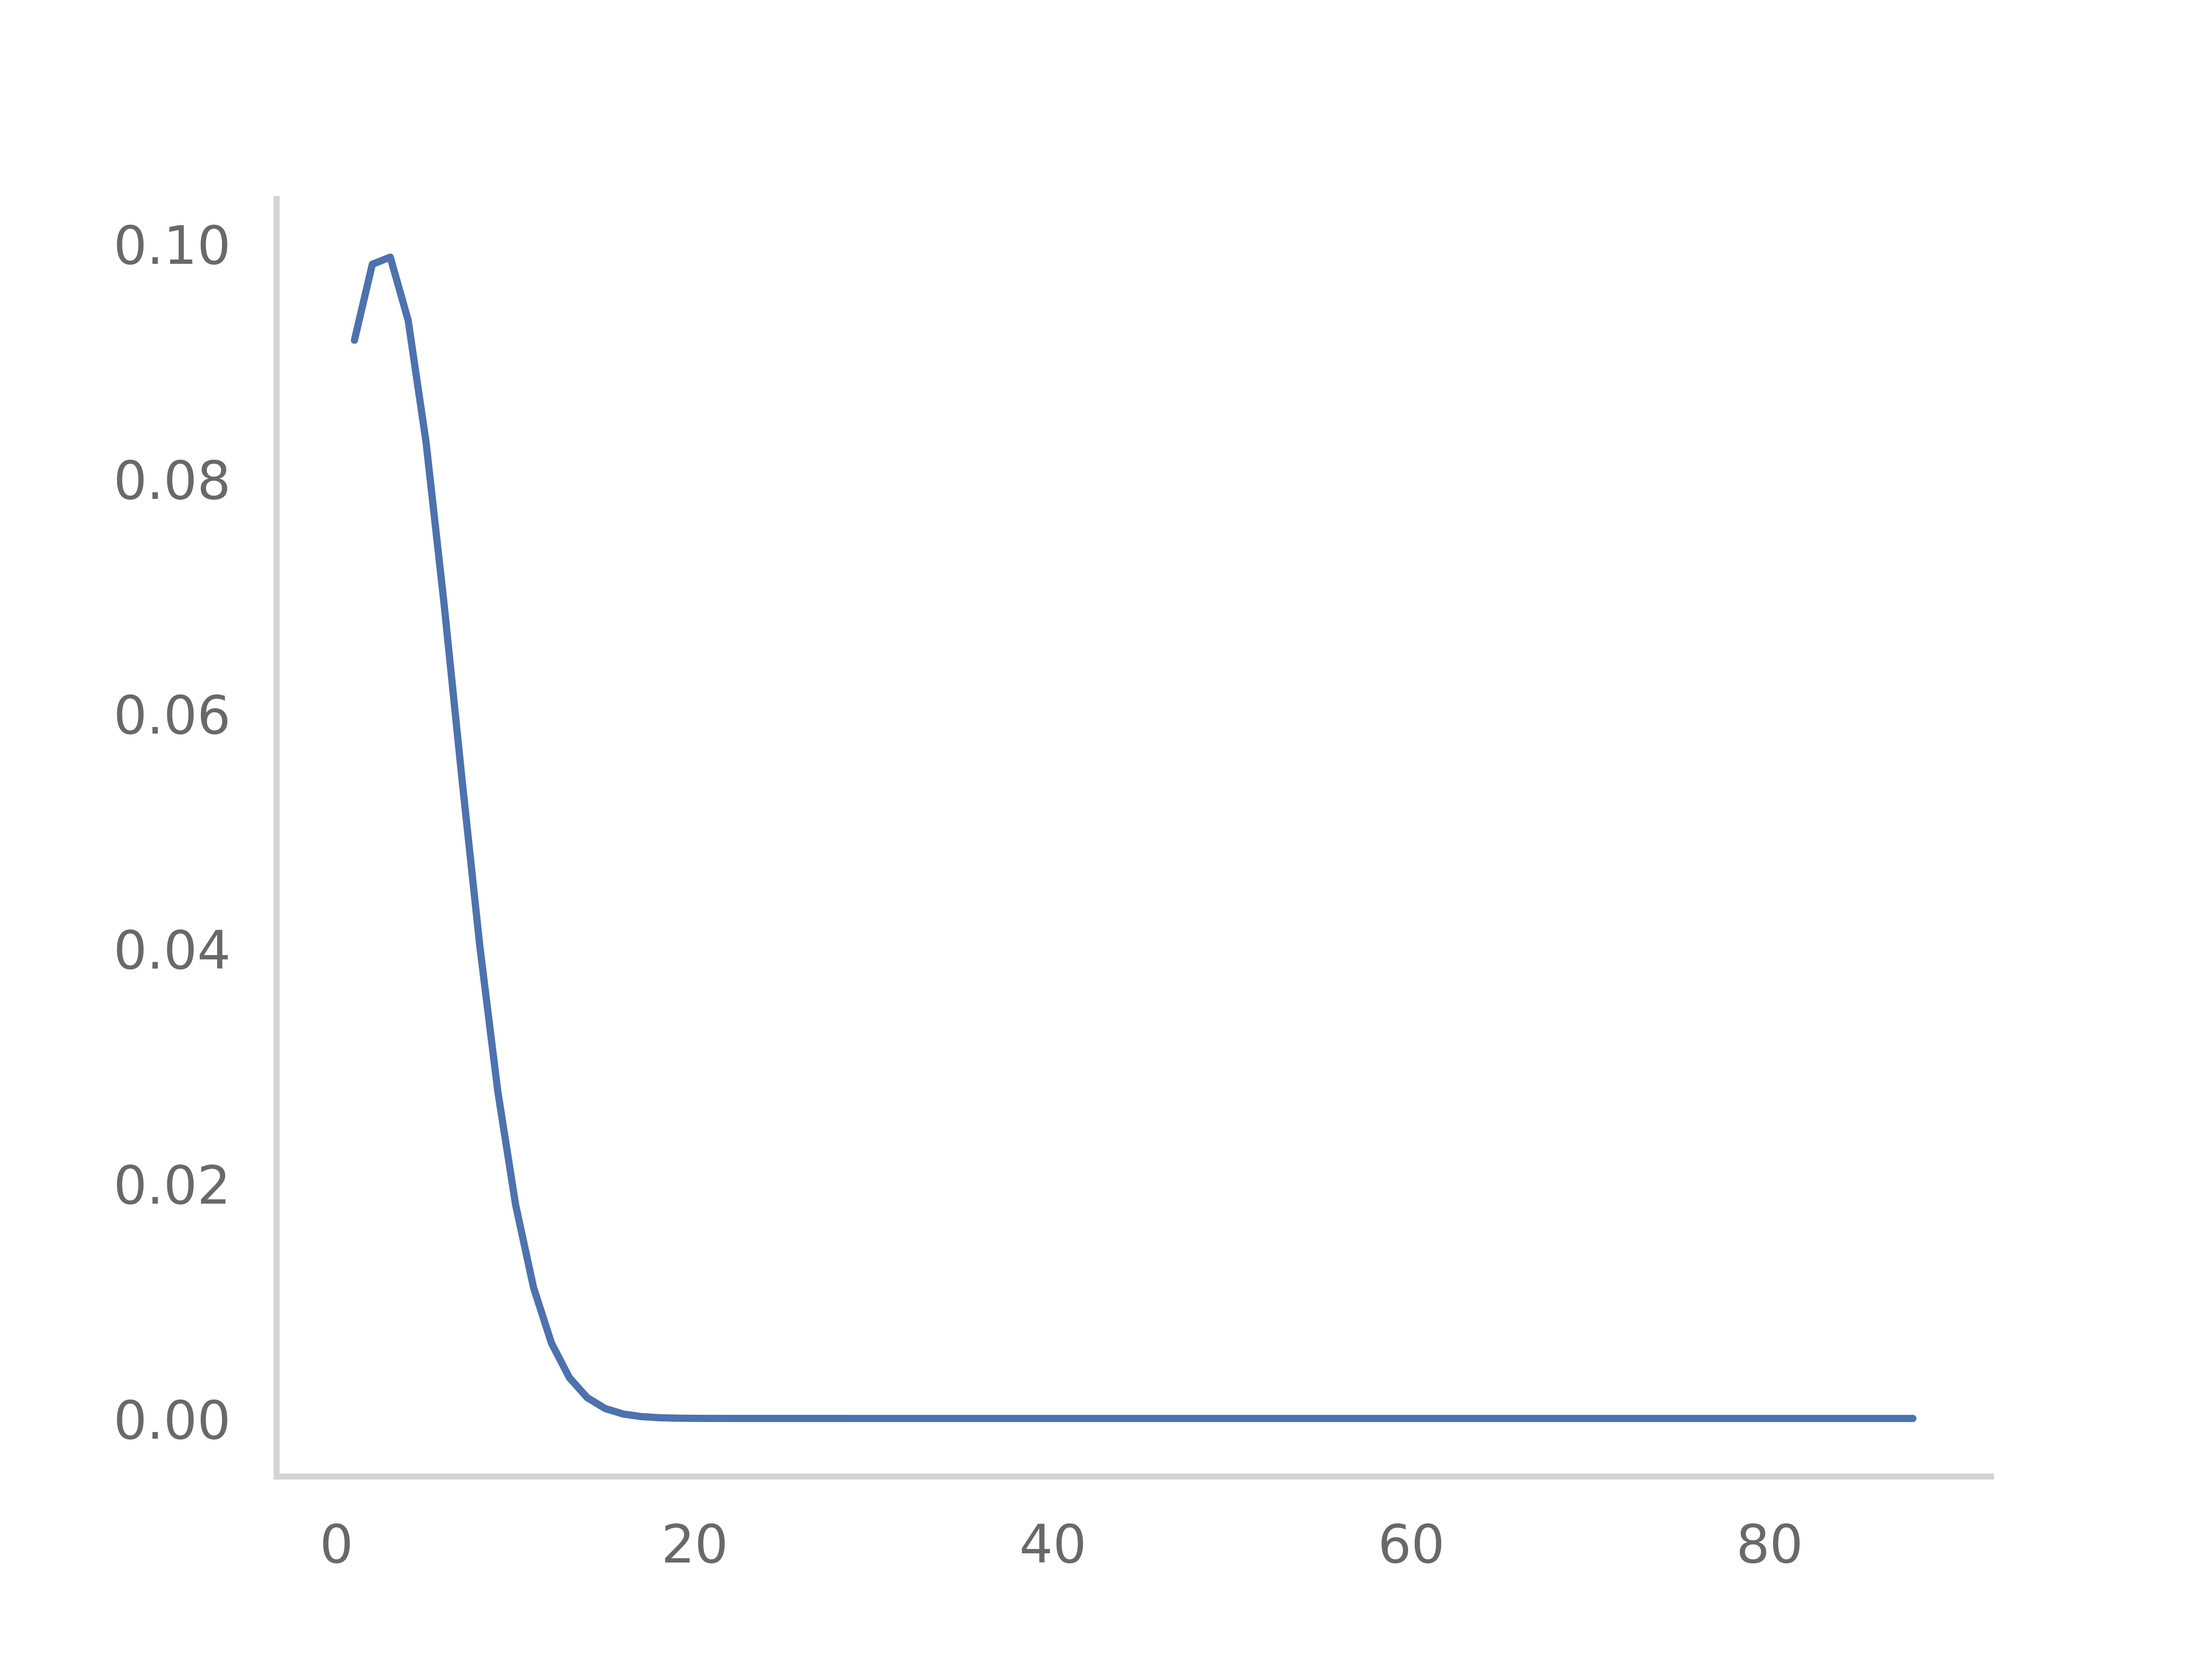
\includegraphics[width=0.85\textwidth]{species_region_invasion_no_filter.png}
%	\label{fig:pdf_invasions}
%    \caption{Probability density function of of the number of invasions.} 
\end{minipage}%
\begin{minipage}{.5\textwidth}
  \centering
    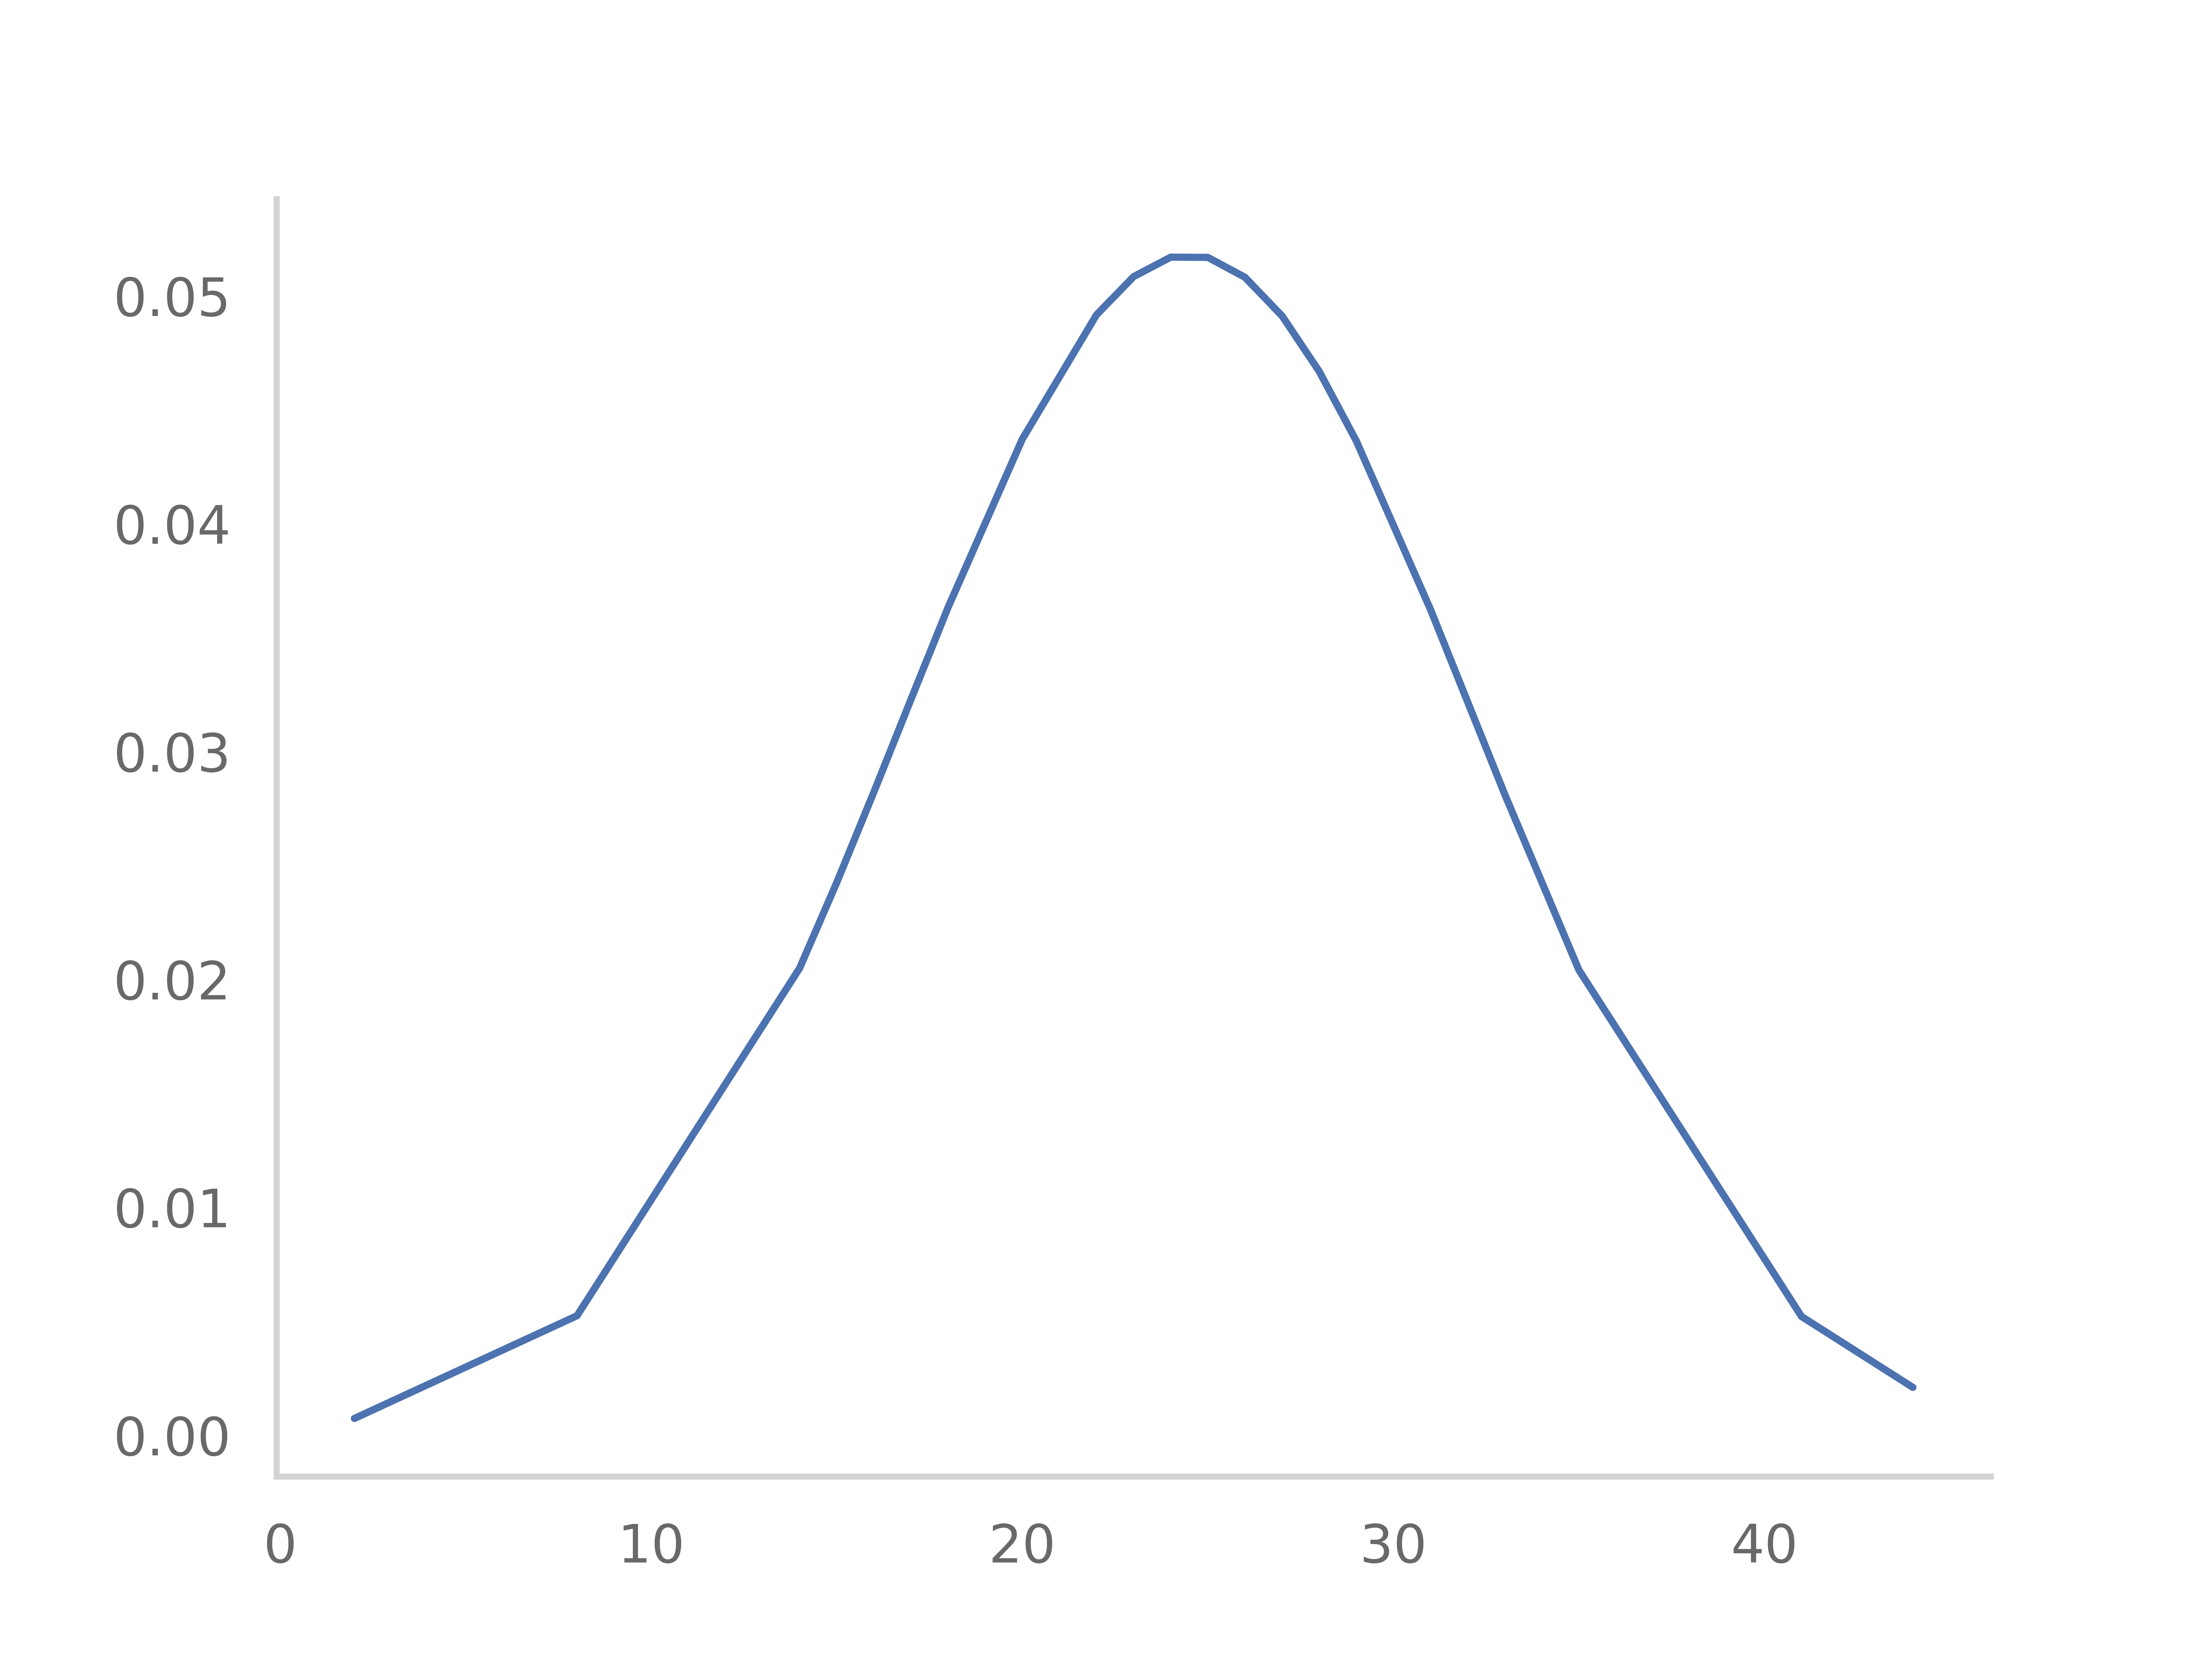
\includegraphics[width=0.85\textwidth]{species_region_invasion.png}
%    \label{fig:pdf_invasions_filtered}
%    \caption{Probability density function of of the number of invasions.}
\end{minipage}
\caption{Probability density function (PDF) of the number of invasions during the entire time frame of the study (1850-2010). The left graph shows that the PDF is strongly left skewed. The second PDF, on the right, is generated after removing all species that did not invade a significant amount of regions.}
\label{fig:pdf_invasion}
\end{figure}

%TODO some closing thoughts?
\chapter{Literature background}

In this section, we cover all the necessary background tools to develop our latent space relational event model. First, we introduce the concept of a latent space model employing a state space model. Then we cover in-depth how to infer this model. We introduce then the reader to the Expectation-Maximization and Kalman Filter algorithms. 

\section{State space model}
\label{sec:latent_space}
%http://www.scholarpedia.org/article/State_space_model

\begin{figure}[H]
    \centering
    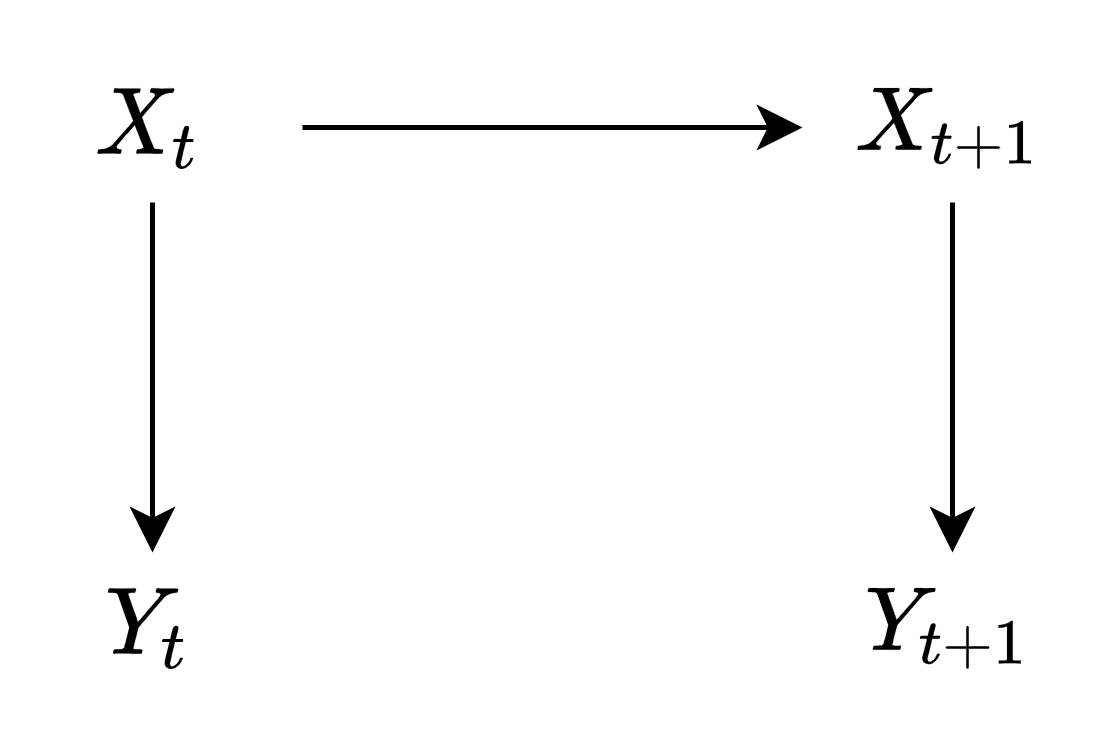
\includegraphics[width=0.35\textwidth]{statespace_diagram.png}
    \caption{State space model diagram representation.}
    \label{fig:statespace_diagram}
\end{figure}

A state-space model is a class of temporal probabilistic models that describe the statistical dependency of latent variables and observed measurement, respectively in the state space $X \in R^d$ and the observed space $Y \in R^m$. In the simplest state-space model, the dynamics are assumed to be a random walk where the jumps between two-time intervals are affected by noise. The first example of such models is the linear Gaussian state-space model, given as follows for $k = [0, ..., n]$

\begin{eqfloat}
\begin{equation}
    \begin{cases}
      x_k = A_k x_{k-1} + \epsilon \; , \quad \epsilon \sim N(0, \Sigma) \\
      y_k = B_k x_k + \delta  \; , \quad \delta \sim N(0, \Delta) 
    \end{cases}\,.
\label{eq:statespace}
\end{equation}
\caption{State space model}
\end{eqfloat}

where the matrix $A \in R^{dxd}$ is the state-transition matrix where $d$ is the dimensionality of the state space $X$. Similarly, $B \in R^{mxm}$ is the observation-transition matrix where $m$ is the dimensionality of the observation space $Y$. The linear Gaussian model can be extended in various ways but in this section, to keep things simple, we focus on the linear Gaussian model. 

The state and observation equations are generally or partially unknown and the parameter $\theta=(A, B, \Sigma, \Delta)$ and $x(k)$ need to be jointly estimated. Maximum likelihood is a well established method in the statistics field to make such parameter estimation. One popular method to estimate state space parameters is the Expectation Maximization algorithm.


\section{Expectation Maximization}
\label{sec:em}

The expectation Maximization (EM), introduced in 1977 by \citet{paper:dempster}, is a family of algorithms that iteratively cycles between two states until convergence is satisfied. In doing so, it first computes the conditional expectation of the complete likelihood and then maximizes it. This approach is really powerful when applied to problems in which a direct calculation of the likelihood $p(y|\theta)$ is computationally unfeasible. Furthermore, we are in particular interested in the application of this family of algorithms to problems where the full data is not available or some variables are latent (see Sec. \ref{sec:latent_space}). \\

The first step called, the expectation procedure (E-step), computes the expectation of the logarithm of the complete data likelihood $Q$

\[
Q(\theta^{(k)}) = E_{x} \left[ log(p(x, y | \theta^{(k)}) \right]
\]

then, with the updated parameter $\theta^{(k)}$ we maximizise $Q$ on the second step, called Maximization step (M-step) and obtain $\theta^{(k+1)}$. The procedure is illustrated in Fig. \ref{em:cycle}. 

\begin{algorithm}[h]
\While{not converged}{
  $\textrm{E-step:} \;  E_x[Q(\theta^{(k)})] $\;
 $\textrm{M-step:} \; \theta^{(k+1)} = \textrm{argmax}_{\theta} \; Q(\theta)$
}
  \label{em:cycle}
  \caption{A general Expectation Maximization framework.}
\end{algorithm}

The computation of the expectation $E[Q(\theta^n)]$ is typically computationally untractable. To make things computationally worse, its complexity increases with the amount of data fed to the model. However, there are many approaches available to estimate this quantity \cite{book:EMBook}. In this thesis, we are interested in an approach to estimate $Q$ called the Kalman Filter.

% ----------------------------------------------------
%TODO more in detail??
%\begin{eqfloat}
%\begin{equation}
%Q(\theta^n) = E_{\theta^n} \left( log(p(x, y | \theta) \right)
%\label{eq:em_expectation}
%\end{equation}
%\caption{Euclidean distance and dot product}
%\end{eqfloat}
%
%
%\begin{eqfloat}
%\begin{equation}
%Q(\theta^n) = E_{\theta^n} \left( log(p(x, y | \theta) \right)
%\label{eq:em_maximization}
%\end{equation}
%\caption{Euclidean distance and dot product}
%\end{eqfloat}


%The key idea of the EM algorithm is that instead of computing the marginal likelihood (which is computationally unfeasible) we compute a lower bound of it. 
%
%\[
%log p(y_{0:T} | \theta) \geq F[q(x_{0:T}, \theta] 
%\]
%
%where $p(y_{0:T} | \theta)$ is the marginal distribution, $q$ is an arbitrary density function and $F$ is a functional defined as TODO. By iteratively maxising the right hand of the equation we can maximise the left hand (i.e. the marginal distribution).  
%
%Given the latent space model in Eq. \ref{eq:latentspace}, a straightforward way to treat the unknown parameter $\theta \in R^d$ would  be to write the full posterior distribution. Unfortunately, this approach is not feasible.
%
%\[
%p(x_{0:T}, \theta | y_{0:T}) = \frac{p(y_{0:T} | x_{0:T}, \theta) p(x_{0:T} | \theta) p(\theta)}{p(y_{0:T})}
%\]


%There exist many other parameter estimation methods for state space models and for more general statistical models, but here we concentrate on these, because these approaches are the most widely used (probabilistic methods) in the state space context.
% ----------------------------------------------------

\section{Kalman Filter}
\label{sec:kalman}

In 1960 R.E. Kalman published his paper describing a recursive solution to the discrete-data linear filtering problem (\citet{paper:kalmanfilter}). Since then, the Kalman filter gained extreme popularity in the machine learning and robotics research field, particularly in the area of autonomous navigation systems. The Kalman filter estimates the evolution of a process by using feedback control. The filter first computes an estimation of the current process state at some time, then, tries to "filter out" the measurement noise in an iterative process. As such, the Kalman filter equations can be subdivided into two categories: the prediction step and the update step. The prediction step is responsible for projecting forward in time the current state of the system. The update step takes the a-prior estimate given from the prediction step and by taking new measurements of the error tries to obtain an improved a-posterior estimate of the state. Indeed, the general form of the algorithm resembles a predictor-corrector algorithm for solving numerical problems. In this chapter, a brief non-technical overview of the Kalman filter is provided. A reader interested in a more in-depth discussion of the formulation of the Kalman filter is advised to read \citet{paper:Maybeck79}.

%A very “friendly” introduction to the
%general idea of the Kalman filter can be found in Chapter 1 of [Maybeck79], while a more complete
%introductory discussion can be found in [Sorenson70], which also contains some interesting
%historical narrative. More extensive references include [Gelb74], [Maybeck79], [Lewis86],
%[Brown92], and [Jacobs93].

\begin{figure}[h]
    \centering
    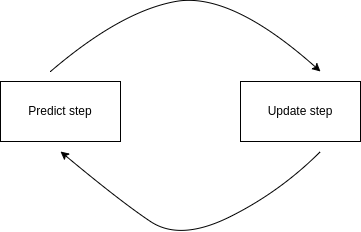
\includegraphics[width=0.25\textwidth]{kalman_diagram.png}
    \caption{The Kalman filter cycle. The time update forwards the current state estimate in time. The measurement update filters the noise out of the projected estimate.}
    \label{fig:kalman_cycle}
\end{figure}

%Let's consider the general problem of trying to estimate the configuration of the state $x \in \mathcal{R}^n$ of a linear process evolution in discrete time
%
%\[
%x_k = A x_{k-1} + v \; , \quad v ~ N(0, \Sigma)
%\]
%
%with a measurement $y_k \in \mathcal{R}^m$ 
%
%\[
%y_k = H_k x_k + w \; , \quad w  ~ N(0, \delta) \\
%\]

%The normal distributed random variables $v, w$ represent noises in the process and in the observation, respectively, and are assumed to be conditionally independent of each other. The matrix $A \in \mathcal{R}^{n, n}$ forwards the state $x_{k-1}$ to the next state $x_k$. The matrix $H \in \mathcal{R}^{m,n}$ relates the measurement $y$ to the process $x$.


We are interested in estimating the configuration of the state $x \in \mathcal{R}^d$ given in equation \ref{eq:statespace}. We consider the initial state $x_0$ as a random vector with a known mean and variance.

\begin{eqfloat}
\begin{equation}
\begin{array}{l}
\hat{x}_0 = \mu_0 = E[x_0] \\
\hat{V}_0 = V_0 = E[(x_0-\hat{x}_0)(x_0-\hat{x}_0)^T] 
\end{array}
\label{eq:linear_kalman_init}
\end{equation}
\caption{Initialization}
\end{eqfloat}


We define $\hat{x}_k^-$ to be our a-priori estimate of the state $x$ at time $k$, given the knowledge of the previous state. Similarly, we define $\hat{x}_k$ to be our a-posteriori estimate at time $k$ given a measurement $y_k$. 

We forecast an update of the estimation of $\hat{x} \approx x$ in time

\begin{eqfloat}[H]
\begin{equation}
\begin{array}{l}
\hat{x}_k^- = A_k \hat{x}_k  \\
\hat{V}_k^- = A_k \hat{V}_k^- A_k^T + \Sigma_k \\
\end{array}
\label{eq:kalman_predict}
\end{equation}
\caption{Prediction step}
\label{eq:linear_kalmann_prediction}
\end{eqfloat}

Where $\Sigma_{t}$ the process noise covariance matrix. 


The goal of the Kalman filter is to express the a-posteriori state $\hat{x}_k^-$ in terms of a linear combination of the a-priori state and the difference between an actual measurement $y$ and a measurement prediction $B \hat{x}_k^-$. 


%\[
%\hat{x}_k = H\hat{x}_k^- + K (y_k - H_k \hat{x}_k^-)
%\]
%\[
%V_k = (I-K_k H_k)V_k^-
%\]

\[
\hat{x}_k = \hat{x}_k^- + K_k (y_k - B_k \hat{x}_k^-)
\]
\[
V_k = (I-K_k B_k)V_k^-
\]



For a statistical motivation, I redirect the reader to \citet{paper:Maybeck79}. The difference $y_t - h_t(\hat{x}_t^-)$ is a residual of the estimation against the measurement, reflecting the error between the predicted measurement and the real measurement. The matrix $K$ is called the Kalman gain matrix and is defined as 


\[
K_k = V_k^- B^T_k (B_k V_k^- B^T_k + R_k)^{-1}
\]


%\[
%K_k = V_k^- H^T_k (H_k V_k^- H^T_k + R_k)^{-1}  \quad , \; H_k = \frac{d}{dx} h(x)
%\]


The Kalman gain matrix goal is to minimize the a-posteriori covariance error matrix $V_t$ at time $t$. With some ease, a way of thinking $K$ is that as the measurement error covariance $R$ is close to zero the measurement $y$ is trusted more and the update is made with high precision. On contrary, if the a-priori estimate error covariance $P^-$ is close to zero, the actual measurement $y$ is less trusted and the predicted measurement $H\hat{x}_t^-$ trust is increased. The "trust" is then reflected in the weights of the Kalman gain matrix $K$.

%Then, on the update step, we filter the noise out of the predicted step a priori estimate and obtain a new estimate $\hat{x}_k$

%\begin{eqfloat}[H]
%\begin{equation}
%\begin{array}{l}
%K_k = V_k^- B^T_k (B_k V_k^- B^T_k + R_k)^{-1} \\
%\hat{x}_k = x_k^- + K (y_k - h(\hat{x}_k^-)) \\
%V_k = (I-K_k B_k)V_k^-
%\end{array}
%\label{eq:kalman_update}
%\end{equation}
%\caption{Update step}
%\label{eq:linear_kalmann_update}
%\end{eqfloat}

The choice of $\Sigma$ is not much deterministic. In a practical way, the noise source $\Sigma$ is often used to capture uncertainty in the process model. Hence, a poor model choice can suffice by simply choosing a large enough uncertainty, by selecting a large covariance $\Sigma$. 


%\begin{eqfloat}
%\begin{equation}
%    \begin{cases}
%      x_k = A x_{k-1} + v \; , \quad v ~ N(0, \Sigma) \\
%      y_k = H_k x_k + w \; , \quad w  ~ N(0, \Sigma) \\
%      \end{cases}\,.
%\label{eq:latentspace}
%\end{equation}
%\caption{Latent space}
%\end{eqfloat}



\chapter{Model}
In the previous section, we introduced to the reader how to make inference on a linear gaussian state space model. In this section, we introduce the REM based on the underlying Alien Species First Records database \cite{intro:dataset}. We first define what the relational events are in our study, how the species and regions are disposed in the latent space, and how to infer it using the Expectation Maximization algorithm and the Kalman filter similarly to as done in the previous section.

\section{Relational event models (REM)}
\label{model:rem}

\citet{rem:butts} proposed a statistical modeling framework capable of analyzing temporal information and the evolution of a sequence of relational events. Given a set of receiver nodes, a set of sender nodes, and a timeframe, a relational event $e$ is a triplet of a sender, a receiver, and a timestamp. Depending on the underlying data, the sender set and receiver set may be the same set or be disjoint sets, depending on the kind of relationship between senders and receivers. In our study of the co-invasion of alien species, the species are the sender and the regions the receivers. Senders and receivers are disjoint sets. This relational event is unidirectional and bipartite. In fact, only a species can invade a region, a region can't invade any other region (or species), and no species-species (or region-region) relational event is allowed. In general, a REM specifies varying distributions for all dyads as a function of past events $E=(e_1, ..., e_N)$ where each event $e_i$ is defined as


\[
e_i = (s_i, r_i, t_i)
\]

In the above notation, $s_i \in S_{t} $ is a sender node (i.e. a species), $r_i \in R_{t}$ a receiver node (i.e. a region) and $t_i$ is the time of the interaction. The sets $S_i, R_i$ respectively contain the receiver and senders nodes.

% The cross product of these two sets is called \textit{risk set} $R_{t_i}$  \footnote{\label{riskset_footnote}To avoid confusion, note that Butts originally called this set the \textit{support set}.}
%
%\[
%R_{t_i} = S_{t_i} \times R_{t_i}
%\]

The risk set $\mathcal{R}_t$ \footnote{To avoid confusion, note that Butts originally called this set the \textit{support set}.} is the set of all dyads for which, at a given timestamp $t$, a relational event can occur.

\[
\mathcal{R}_{t} = \{(s,r) \; | \; \textrm{may occurs} \; \textrm{at} \; t_i\}
\]

The waiting time $T_{s,r}$ for a particular dyad to happen between a species $s$ and a region $r$ is assumed to be exponentially distributed 

\[
T_{s,r} \sim Exp(\lambda(s, r, t)
\]


In the above equation, the hazard function $\lambda$ is defined as

\[
\lambda(s, r, t) = \lim_{\delta t \lim 0^+} \frac{P(t \leq T_{s,r} \leq t + \delta t | t \leq T_{s,r})}{\delta t}
\]

The hazard function can be interpreted as the expected number of relational events in a time interval of length one, conditionally on the previous network events. The most commonly used hazard function is the Cox proportional hazard model. 

%%Theta is what thet called beta in Igor's paper (change it?)

\[
\lambda(s, r, t) = \lambda_0(t) \cdot exp({X_{sr}^{(t)} \beta} )
\]

In this equation, $\lambda_0$ represents a baseline hazard for all dyads in the risk set $\mathcal{R}$. Instead, the variable $X_{sr}^{(t)}$ is some dyadic covariate at time $t$. To estimate the parameters $\beta$ we maximize the partial likelihood of the Cox proportional hazard model 


\[
L(\beta) =  \prod_{i=1}^n \frac{exp (X_{s_i r_i}^{(t_i)} \beta) }{ \sum_{(s,r) \in \mathcal{R}_{t_i}} exp({X_{sr}^{(t_i)} \beta} )}
\]

if the time is considered to be continuous. In a discrete time scenario, the parameter $\beta$ can be estimated in a more straightforward way by maximising the Poisson likelihood by a linear regression:

\[
L(\beta) =  \prod_{i=1}^n P(Y_k | \lambda_k)
\]


Typically the research interest is to estimate the factors that increase, or decrease, the likelihood $L$, more specifically, the parameter $\beta$.


\section{Latent space REM}
 
%Maybe better to introduce the counting process before, y is the count 

Every invasion of a species $s \in S$ and region $r \in R$, where $S, R$ are respectively the sets of species and regions in the dataset, can be modeled as a multivariate Poisson counting measure  $N$.

\[
N_t(s, r) = \textrm{number of invasions} \; e \; in \; interval \; [0, t]
\]

An alien species is not allowed to leave a region after an invasion has happened and, eventually, invade it a second time. Therefore, an invasion can happen only once. The counting process $N$ is therefore bounded by 1. We define $T(s, r)$ to be a function that returns the time of invasion for specie $s$ an region $r$. The function $N$ can either take a value of one or zero depending on whether an invasion happened previously to $t$ for a determined region and species.


\begin{eqfloat}
\begin{equation}
\begin{array}{l}
N_t(s, r) = 0 \; if \; t < T(s, r) \\
N_t(s, r) = 1 \; if \; t >= T(s, r)
\end{array}
\label{eq:counting process}
\end{equation}
\caption{The counting process $N$ is either 0 or 1 depending if an alien species has invaded or not a country.}
\end{eqfloat}

% Introduce the latent space

We dispose our actors, which are species and regions, into a latent space $X \in \mathcal{R}^n$. Each actor is assigned a position inside $X$. It is worth mentioning, to avoid confusion, that these positions in $X$ are disconnected from the real world. The closeness of two actors in the latent space $X$ does not imply their closeness on the world map. We then define $Y$, the observed state. In our study, the observed state is the observed count of invasions modeled as Poisson. Similarly to the state space model in Eq. \ref{eq:statespace}, we define

\begin{eqfloat}
\begin{equation}
    \begin{cases}
      x_k = x_{k-1} + \epsilon \; , \quad \epsilon ~ N(0, \Sigma) \\
      y_k \sim Poi(\lambda_k) \; , \quad \lambda^{s, r, k} = exp\left(\alpha-dist(x_s(k), x_r(k)) \cdot \lambda_1(k) \right) \cdot I
    \end{cases}\,.
\label{eq:latentspace}
\end{equation}
\caption{Latent space}
\end{eqfloat}

for $k = [0, ..., n]$. The rates $\lambda$ are censored by multiplying them by the matrix $I$ after an invasion occurs. The matrix $I$ entries are either one or zero depending on if an invasion has occurred.
\[
I_{s,r} = T(s,r)
\]

Without loss of generality, we assume that relational events happen at discrete time intervals. The dynamics of the latent space can be modeled as a random walk where the length of the jumps is dependent on the variance $\Sigma$.


The position $x$ of each vector in the latent space $X$ is constrained by the distance to all the other vectors inside $X$. The distance in this space represents an affinity of each species $s$ to create a connection (i.e. to invade) a region $r$ in the REM. The structure of the latent space $X$ is therefore driven by the similarity between the nodes $s, r$. We expect species that tend to co-invade the same regions to be close in the latent space. Analogous, regions invaded by the same group of species should be near. We are interested in studying the structure of the latent space $X$ to infer which group of species has the tendency to co-invade regions.

% How are the dynamics of N modeled

The observed counts $y$ are a result of the dynamics of the actor's positions and interactions in the REM and latent space $X$. The stochastic intensity of the counting process $N$ is modeled by the function $\lambda$. Heuristically, we assume that the rates $\lambda$ are functions of the distance between species $x_s(t)$ and regions $x_r(t)$ in the latent space (Eq. \ref{eq:latentspace}). 

% Discussion on the distance
Distances between vectors are defined in many different ways. Two main popular choices are euclidean distance and dot product. These two distances give a different interpretation to the model. 

\begin{eqfloat}
\begin{equation}
\begin{array}{l}
dist_{euc}(u, v) = \sum_{i=0}^d |u_i - v_i|^2 \\
dist_{dot}(u, v) = u \cdot v
\end{array}
\label{eq:distance_latentspace}
\end{equation}
\caption{Euclidean distance and dot product}
\end{eqfloat}

We chose the distance in the vector space $X$ to be the dot product. The Euclidean distance imposes a geometric interpretation. In contrast, the dot product yields a spherical structure to the data. We expect the species-region similarities to be better described by the latter.

\begin{eqfloat}
\begin{equation}
\lambda^{s, r, k} = exp\left(\alpha-(x_s(k) \cdot x_r(k)) \cdot \lambda_1(k) \right) \\
\label{eq:ourmodel_lambda}
\end{equation}
\caption{Lambda rates are in function of the distance given by the dot products of vectors in the latent space $X$.}
\end{eqfloat}

\section{Inference}
% Introduce EM for the problem
To infer on the structure of the latent space $X$, and the parameters $\theta$  and $\Sigma$ we use the Expectation Maximization (EM) algorithm (\ref{sec:em}). Since the latent state $X$ is not observed, direct optimization of the maximum likelihood is not possible. We aim to maximise the $\int_x L(\theta, \Sigma ; y, x) dx$. As explained in the background section \ref{sec:em}, the EM instead of directly maximizing this integral, it iteratively computes and maximizes an estimate $Q$ of the parameters $\theta, \Sigma$ conditioned on the previous estimate. 

%TODO a little unclear
\begin{eqfloat}
\begin{equation}
Q(\beta^{n}, \Sigma^{n}) = E_{x|y} \left( log(p(x, y | \beta^{n-1}, \Sigma^{n-1}) \right)
\end{equation}
\caption{Expectation Maximization.}
\label{eq:expectation_maximization}
\end{eqfloat}

where $\beta$ are the remainder parameters related to the covariates and $\theta$ estimates the volatility of the latent process.

% E-step hard to solve -> Kalman filter

\subsection{Extended Kalman Filter}

In section \ref{sec:kalman} we showed how to apply a Kalman filter to solve the E-step of an Expectaction Maximizaton problem of a Linear Gaussian model, but our process $y$ is not linear. We can rewrite the latent space formulation in Eq. \ref{eq:latentspace} slightly differently

\begin{eqfloat}
\begin{equation}
    \begin{cases}
      x_k = f(x_{k-1}) + \epsilon \; , \quad \epsilon ~ N(0, \Sigma) \\
      y_k = h(x_k) 
    \end{cases}\,
\label{eq:latentspace2}
\end{equation}
%\caption{Latent space}
\end{eqfloat}

here $f = I$ and $h$ is a function dependent on the latent space $x$. The function $h$ is not linear because it is a Poison distribution, however, providing that $h, y \in C^1$, we can linearise the process around the mean and reconduct the problem to the basic linear case. By assuming that a step in time in the latent state can be approximated by the conditional distribution 

\[
x_{k} \sim N( \hat{x}_k, \hat{V}_k)
\]

the predict step of the Kalman filter estimates the first two moments of $x_k$. 

\[
\hat{x}_k = E[\hat{x}^-_k]
\]
\[
\hat{V}_k = V[\hat{x}^-_k]
\]

Where $\hat{x}^-_k$  is an a-priori distribution of the state $x$ at time $k$, given the knowledge of the previous state. Hence, by exploiting the natural formulation of our latent space model (Eq. \ref{eq:latentspace}) we can solve the computationally challenging E-step by means of a Kalman filter by approximating the quantity $Q$ in function of its first two conditioned moments $E$, $V$. 

The initial state $x_0$ is a random vector with a known mean and variance.

\begin{eqfloat}
\begin{equation}
\begin{array}{l}
\hat{x}_0 = \mu_0 = E[x_0] \\
\hat{V}_0 = V_0 = E[(x_0-\hat{x}_0)(x_0-\hat{x}_0)^T] 
\end{array}
\label{eq:kalman_init}
\end{equation}
\caption{Initialization}
\end{eqfloat}

We forecast an update of the estimation of $\hat{x} \approx x$

\begin{eqfloat}[H]
\begin{equation}
\begin{array}{l}
\hat{x}_k^- = \hat{x}_{k-1} \\
\hat{V}_k^- =  V_{k-1} + \Sigma
\end{array}
\end{equation}
\caption{Prediction step}
\label{eq:ext_kalmann_prediction}
\end{eqfloat}

We now express the a-posteriori estimation $\hat{x}_k^-$ in terms of a linear combination of the a-priori state and the difference between an actual measurement $y$ and a measurement prediction $h(\hat{x}_k^-)$ state. 

\[
\hat{x}_k = \hat{x}_k^- + K (y_k - h(\hat{x}_k^-))
\]
\[
V_k = (I-K_k H_k)V_k^-
\]

We define the Kalman gain matrix $K$ as 

\[
K_k = V_k^- H^T_k (H_k V_k^- H^T_k + R_k)^{-1}  \quad , \; H_k = \frac{d}{dx} h(x)
\]


We know updated the a-priori estimates of the mean and variance in Eq. \ref{eq:ext_kalmann_prediction} with the observation of state $y$

%\begin{eqfloat}[H]
%\begin{equation}
%\begin{array}{l}
%K_k = V_k^- H^T_k (H_k V_t^- H^T_k + R_k)^{-1} \\
%\hat{x}_k = x_k^- + K_k (y_k - h(\hat{x}_k^-)) \\
%V_k = (I-K_k H_k)V_k^-
%\end{array}
%\end{equation}
%\caption{Update step}
%\label{eq:ext_kalmann_update}
%\end{eqfloat}

By combining equations (\ref{eq:ext_kalmann_prediction}), (\ref{eq:ext_kalmann_update}) we get an algorithm for the Extended Kalman. \\

\begin{algorithm}[H]
\textbf{Initialize: }
\begin{substeps}
$\hat{x}_0 = \mu_0 = E[x_0]$ \;
$\hat{V}_0 = V_0 = E[(x_0-\hat{x}_0)(x_0-\hat{x}_0)^T]$  \;
\end{substeps}
\For{k=1,...,n}{
  Prediction step (Eq. \ref{eq:ext_kalmann_prediction})
  \begin{substeps}
	$\hat{x}_k^- = \hat{x}_{k-1} $ \;
	$\hat{V}_k^- =  V_{k-1} + \Sigma $\;
  \end{substeps}
  Update step (Eq. \ref{eq:ext_kalmann_update})
  \begin{substeps}
	$K_k = V_k^- H^T_k (H_k V_t^- H^T_k + R_k)^{-1}$ \;
	$\hat{x}_k = x_k^- + K_k (y_k - h(\hat{x}_k^-))$ \;
	$V_k = (I-K_k H_k)V_k^-$ \;
  \end{substeps}
}
  \caption{Extended Kalmann Filter}
  \label{algo:ext_kalmann}
\end{algorithm}

% --------- Smoother --------------------
After $n$ iterations of the Extended Kalman Filter are performed, we move backward from the last prediction to the starting point $x_0$ with the goal to update and correct the predictions given by the Extended Kalman Filter. A popular smoother choice is the Rauch-Tung-Striebel smother. 

\begin{algorithm}[H]
\For{k=n...1}{
  $B_k = V_{k-1} V_{k-1}^{-1}$ \;
  $\hat{x}_{k-1} = x_{k-1}^- + B_k (\hat{x}_k - x_{k}^-)$ \;
  $V_{k-1} = \hat{V}_{k-1}^- + B_K (V_k - \hat{V}_k^-)B^T_k $ \;
}
  \caption{Smoother}
  \label{algo:smoother}
\end{algorithm}

\section{Closed form Algorithm}
% --------- M-step --------------------
We now propose a close form for an algorithm based on the Expectation Maximization framework (Eq. \ref{eq:expectation_maximization}) to make inference on our latent space REM. We approximate the E-step through an Extended Kalman Filter proposed in the previous section, then we maximize $Q$. For a number $s$ of steps, we report our model in a closed form


\begin{algorithm}[H]

\textbf{Initialize: }
\begin{substeps}
$\hat{x}_0 = \mu_0 = E[x_0]$ \;
$\hat{V}_0 = V_0 = E[(x_0-\hat{x}_0)(x_0-\hat{x}_0)^T]$  \;
\end{substeps}
\While{not converged}{
  \textbf{E-Step}: 
	\begin{substeps}
	Kalman Filter  (Alg. \ref{algo:ext_kalmann}) \; 
	Smoother (Alg. \ref{algo:smoother}) \;
	\end{substeps}  	
  \textbf{M-Step:}
	\begin{substeps}
	$\beta = \textrm{argmax}_{\beta} Q$ \; 
	\end{substeps}  	
}
\caption{Lantet space REM inference.}
\label{algo:rem_latent}
\end{algorithm}


%\subsection{Model computational complexity discussion}
%TODO brief talk on model complexity

%\subsection{Implementation specifications}
%We implemented the method discussed in TODO section in Tensorflow (TODO add cite) 
%
%%%TODO what framework do we use - how we solved the computational cost problem
%The size of the dataset is problematic under a computational point of view. In particular, the inversion of the matrix TODO and the memory requirements to allocate all the dataset are large. However, due to the filtering described in the previous section and using efficient data structure by saving in memory only the non-zero entries and the indexes in a sparse matrix and by using CUDA toolokits to accelerate the computation in GPU our implementation meets the computational requirements.

\chapter{Results}

In this section, we analyze the results from fitting our model on $15947$ alien species invasions from $1850$ to $2010$, as described in Section \ref{sec:dataset}. In the dataset, there are $1724$ species and $153$ regions. To report the results in the clearest way, we decided to distinguish the region and spaces nodes in the latent space. In Fig. \ref{fig:latentspace_config} the initial and final configuration of the latent space is reported for species and regions. 

Unfortunately, due to the high number of nodes, it is hard to see the evolution of the latent space. In Fig. \ref{fig:latentspace_afew} we focus on a set of 25 randomly chosen nodes to highlight the dynamics of nodes in the latent space. The nodes that tend to have similar behavior (i.e. have the tendency to co-invade) will move towards each other. In contrast, nodes that express a contrary behavior will push each other further. The black arrows show the trajectory in time. There are 17 timesteps in total (the years from 1850 to 2010). Some trajectories are linear and others are elliptic. Species that move with the same trajectory in the latent space will have a tendency to co-invade regions, similarly, regions that move with the same trajectory are more likely to be invaded by the same group of species.


\begin{figure}[H] 
  \begin{minipage}[b]{0.5\linewidth}
    \centering
    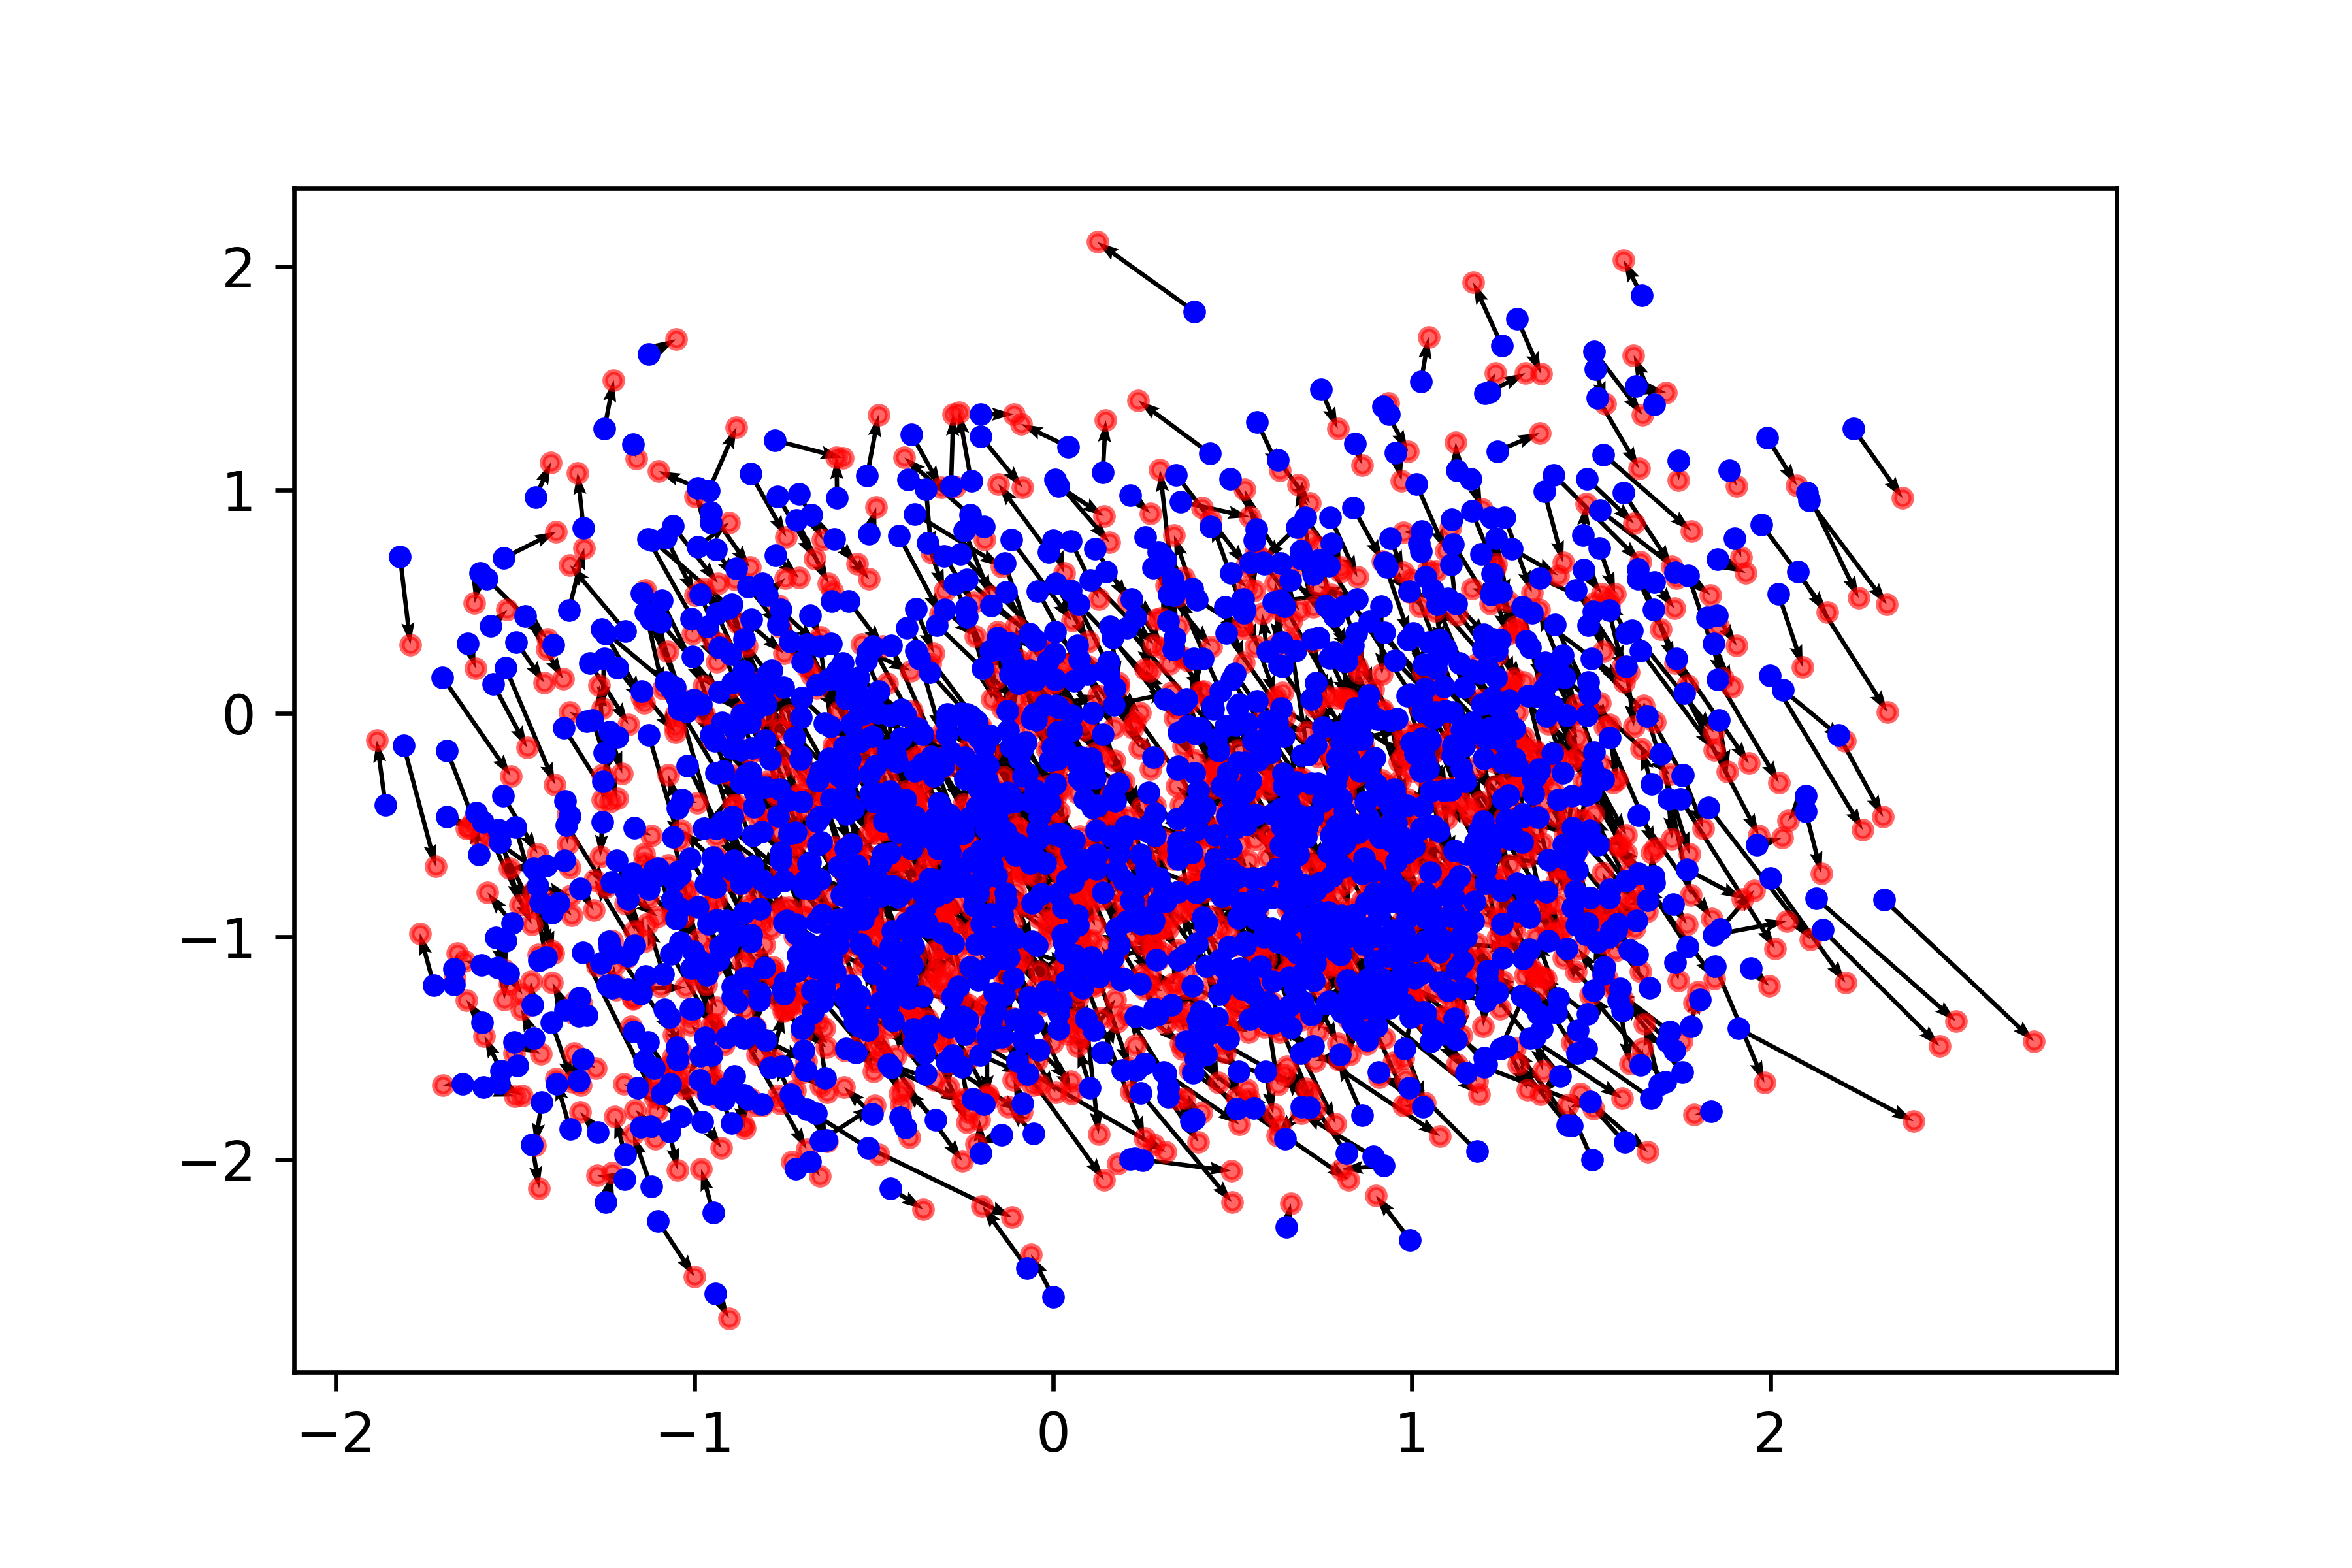
\includegraphics[width=\linewidth]{latentspace_species.png} 
    \vspace{4ex}
  \end{minipage}%%
  \begin{minipage}[b]{0.5\linewidth}
    \centering
    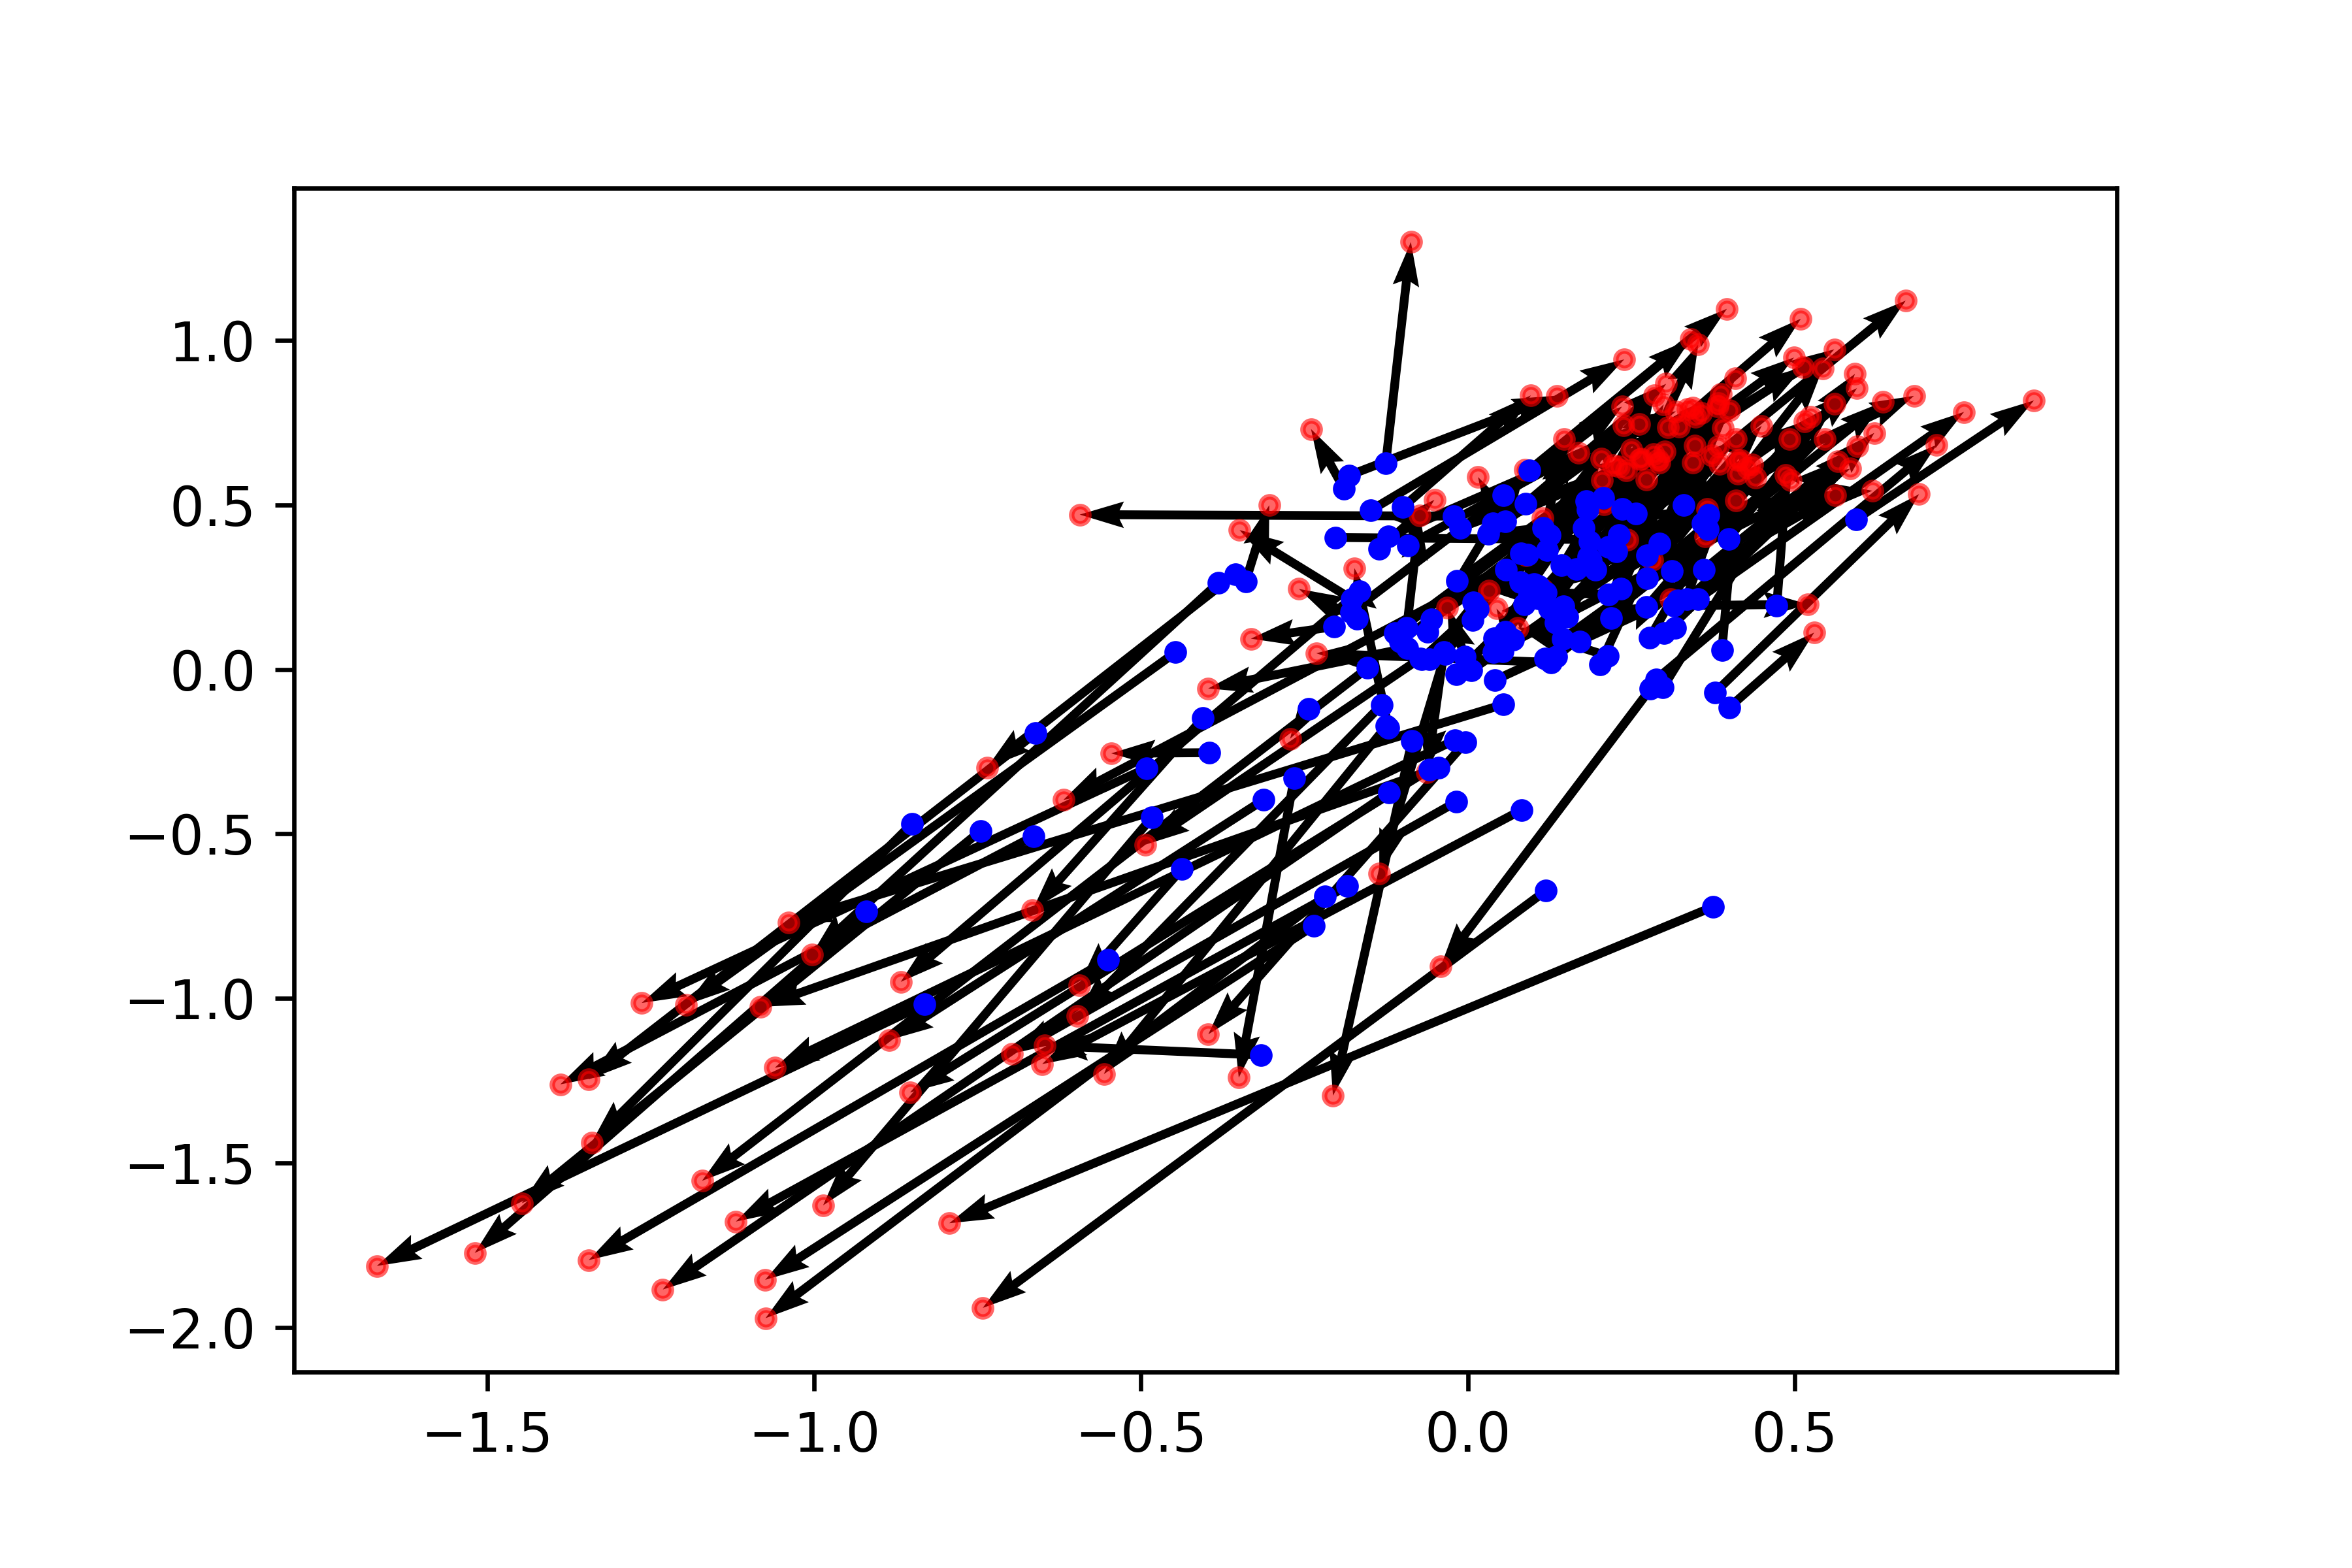
\includegraphics[width=\linewidth]{latentspace_region.png} 
    \vspace{4ex}
  \end{minipage}  
\caption{Latent space initial and final configurations. The black arrows shows the movement in space from the initial state to the final state.}
\label{fig:latentspace_config}
\end{figure}

%TODO select switzerland alongside the random regions
\begin{figure}[H] 
  \label{ fig7} 
  \begin{minipage}[b]{0.5\linewidth}
    \centering
    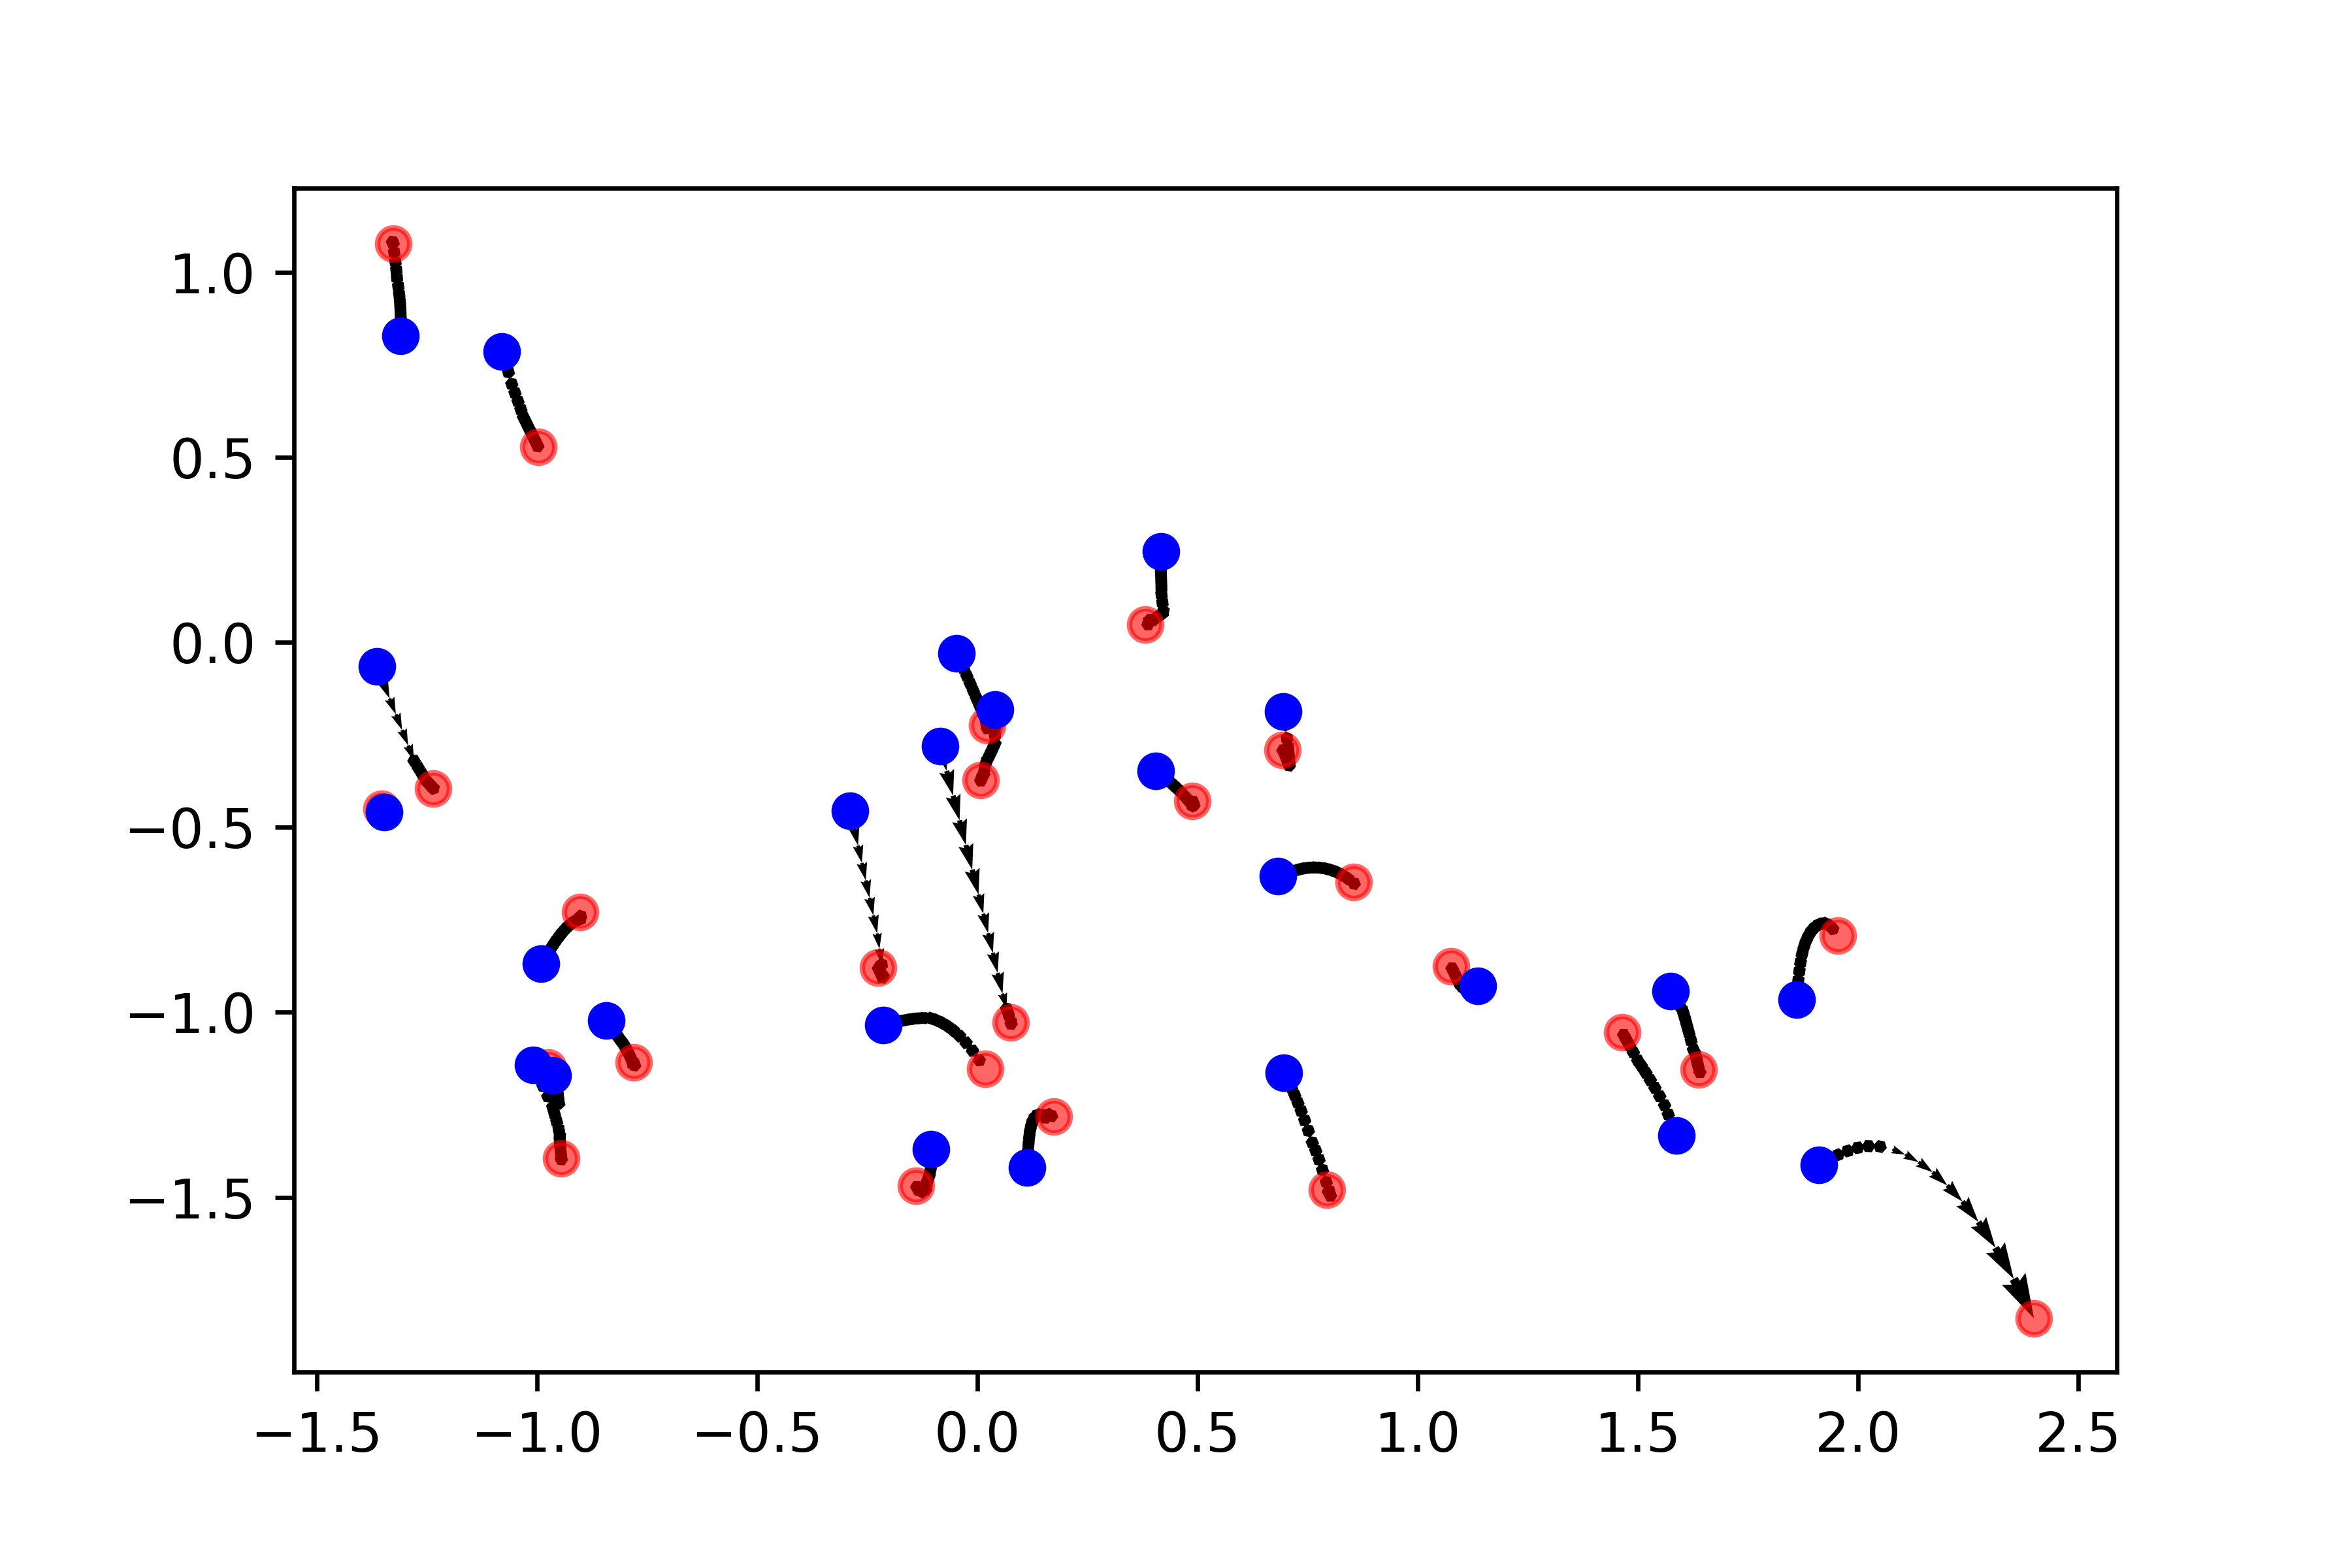
\includegraphics[width=\linewidth]{latentspace_afew_species.png} 
    \vspace{4ex}
  \end{minipage}%%
  \begin{minipage}[b]{0.5\linewidth}
    \centering
    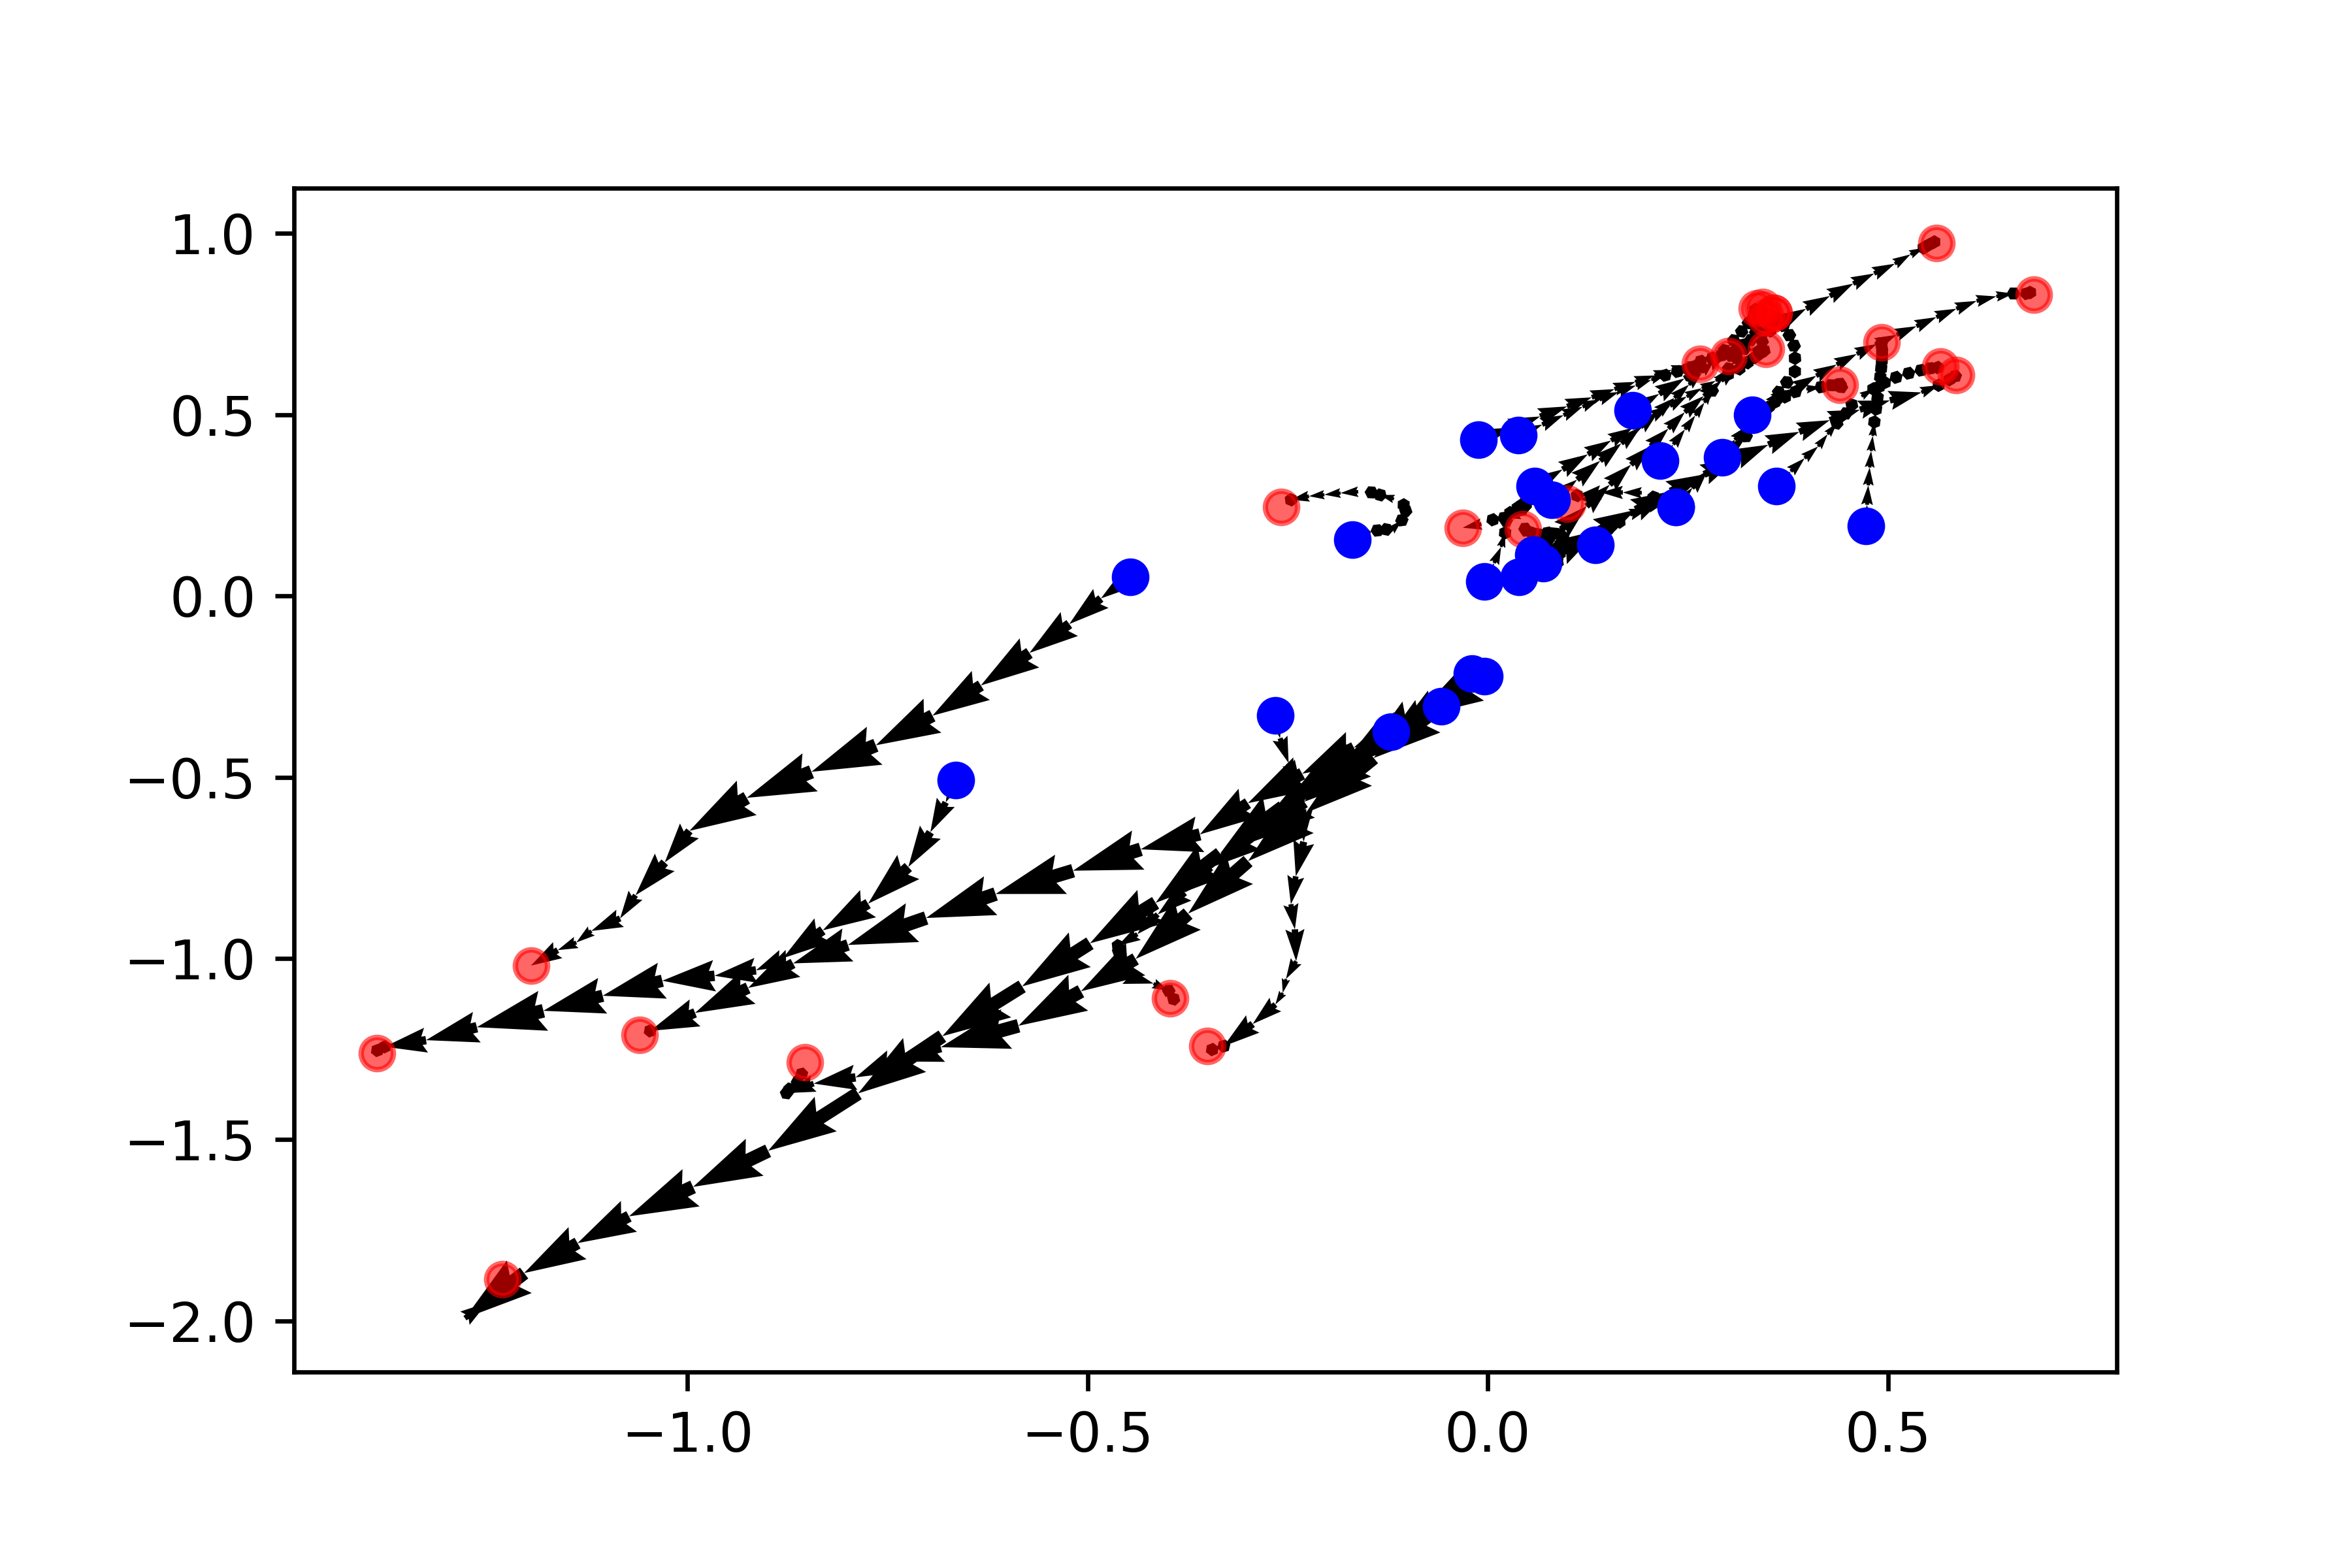
\includegraphics[width=\linewidth]{latentspace_afew_region.png} 
    \vspace{4ex}
  \end{minipage}  
\caption{A set of 25 randomly chosen species (left) and regions (right) and their dynamics in the latent space.}
\label{fig:latentspace_afew}
\end{figure}

\begin{figure}[H]
    \centering
    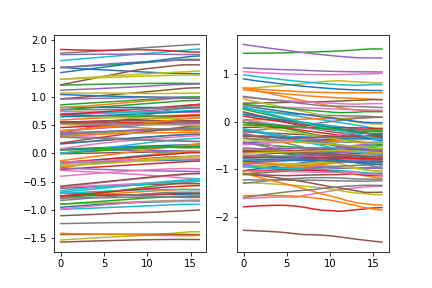
\includegraphics[width=0.75\textwidth]{trajectories_species.png}
    \caption{Plot of the evolution of trajectories in time for 100 randomly selected species. The left image is for the X coordinate, the right image for the Y coordinate.}
    \label{fig:trajectories_species}
\end{figure}

In Fig. \ref{fig:trajectories_species} and \ref{fig:trajectories_region} the trajectories in the latent space by 100 randomly selected species and regions are reported. An in-depth look at these trajectories suggests that there are patterns in the movements of regions and species in the latent space. The trajectories of nodes in the latent space correspond to the co-invasion of species into regions. We now focus our interest on analyzing these patterns in the trajectories. 


\begin{figure}[ht]
    \centering
    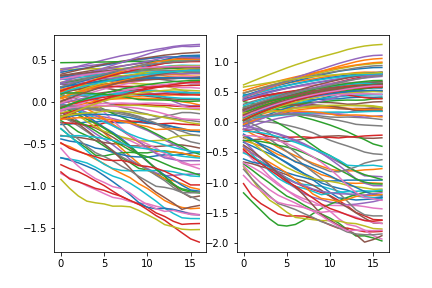
\includegraphics[width=0.75\textwidth]{trajectories_region.png}
    \caption{Plot of the evolution of trajectories in time for 100 randomly selected regions. The left image is for the X coordinate, the right image for the Y coordinate.}
    \label{fig:trajectories_region}
\end{figure}

Species that move in a similar way inside the latent space tend to co-invade. Similarly, regions that move analogously will have the tendency to be co-invaded by the same group of species. To detect nodes that move in a homogeneous way we decided to use a clustering algorithm. We settled on using a \textit{Ordering points to identify the clustering structure} (\textbf{OPTICS}) algorithm to perform the clustering. OPTICS is a variation of the DBScan clustering algorithm, which an in-depth cover is out of the scope of this thesis. This algorithm is really similar to DBSCan but addresses one of the major flaws of the algorithm. DBSCan does not perform very well on data with a non-uniform density. 

Applying OPTICS to the species and regions in the latent space detected 67 clusters for species and 5 clusters for regions \ref{fig:cluster_density}. The dynamics of the clusters are reported in Fig. \ref{fig:latentspace_cluster} with all the nodes not belonging in any cluster greyed out. 

\begin{figure}[H] 
  \begin{minipage}[b]{0.5\linewidth}
    \centering
    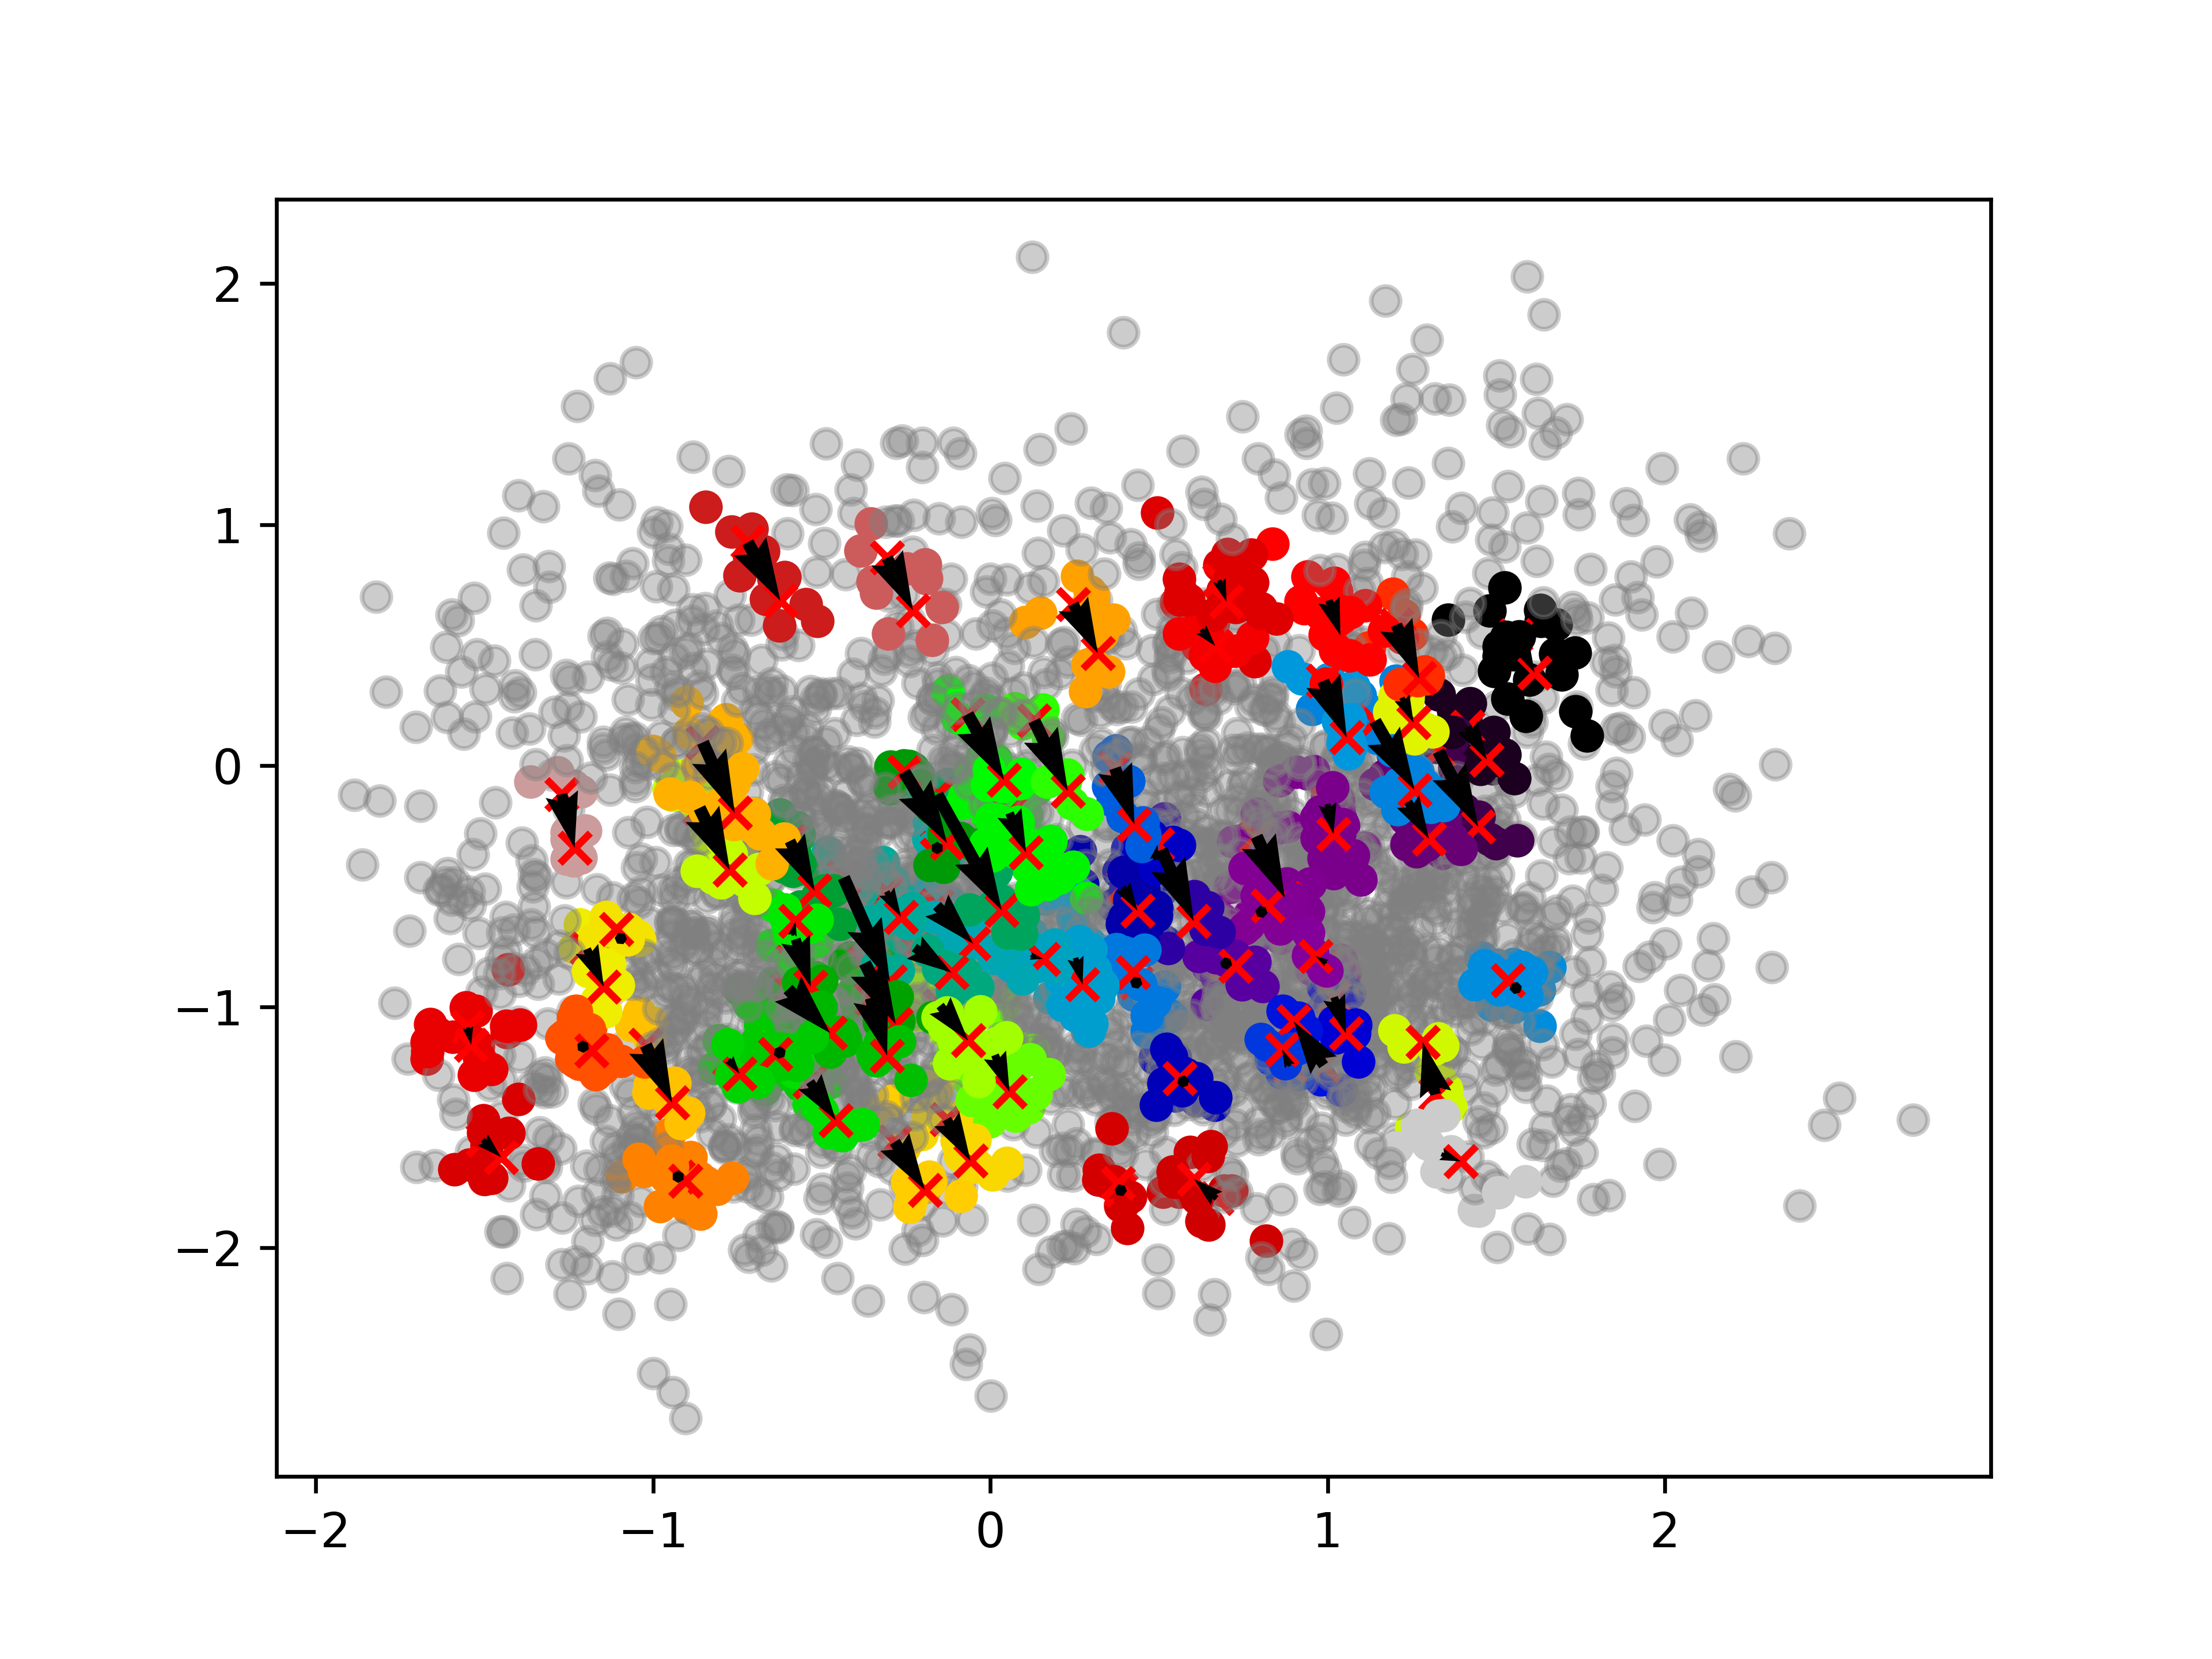
\includegraphics[width=\textwidth]{latentspace_cluster_species.png}
    \vspace{4ex}
  \end{minipage}%%
  \begin{minipage}[b]{0.5\linewidth}
    \centering
    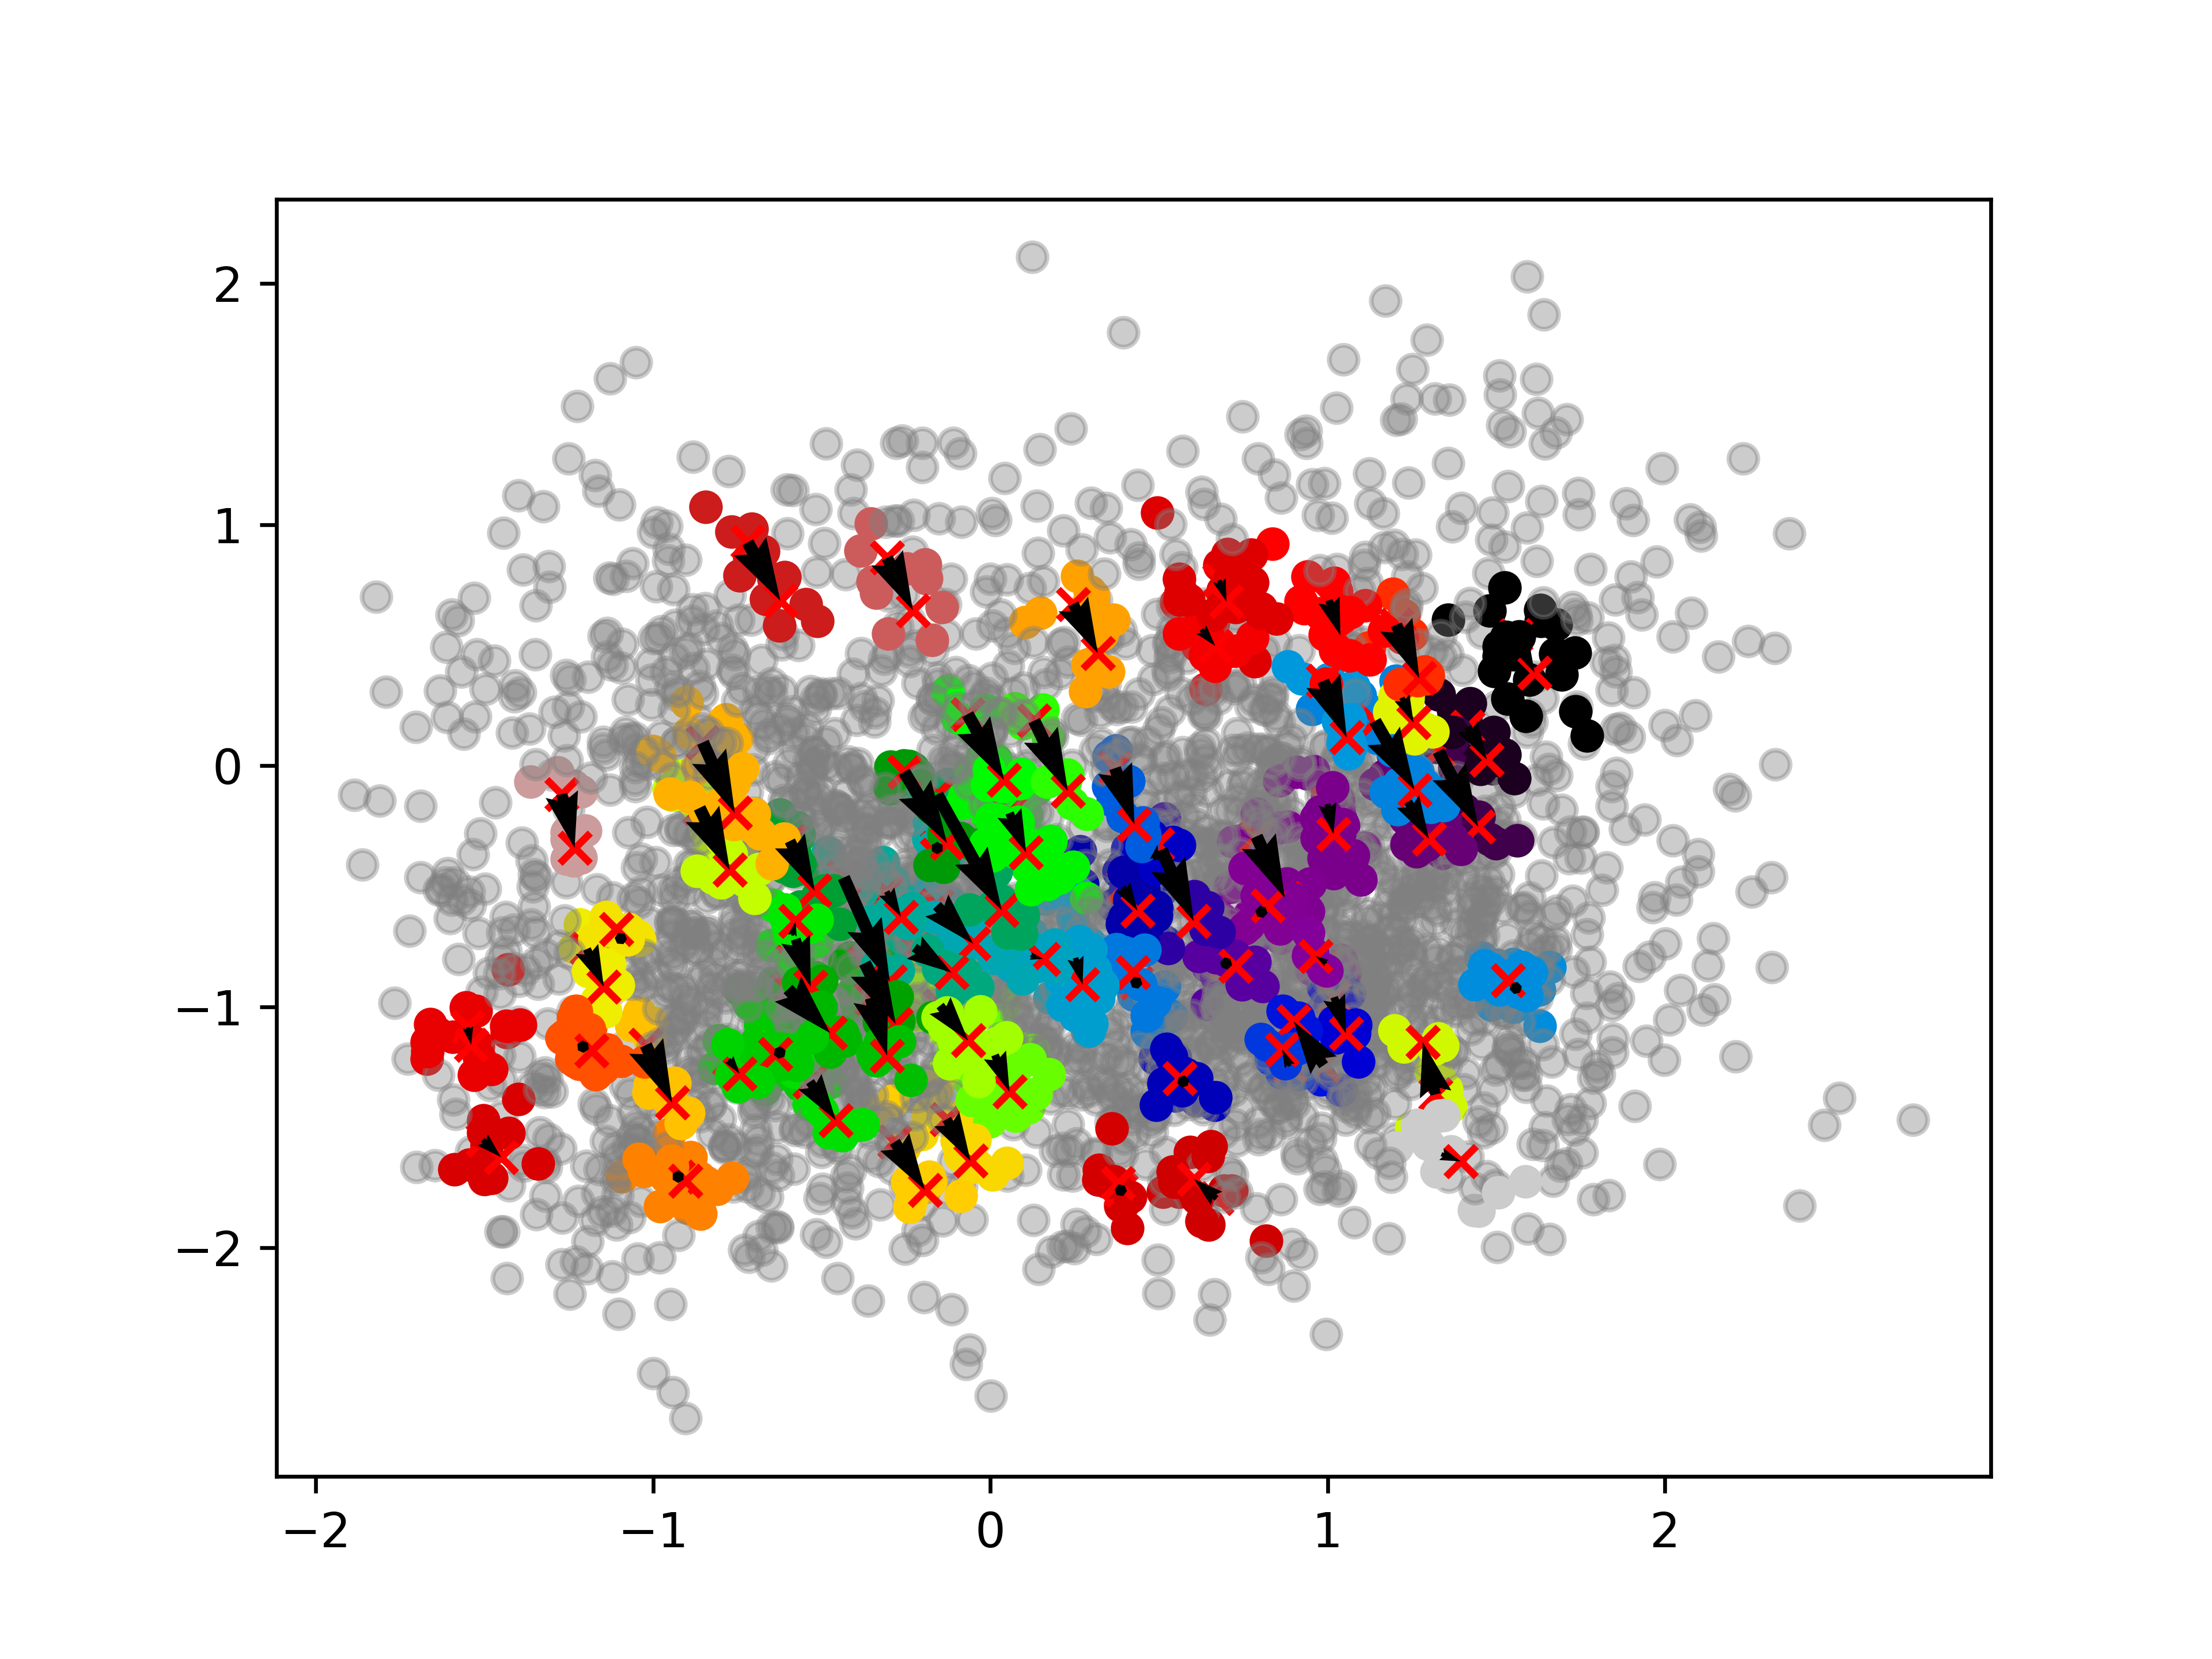
\includegraphics[width=\textwidth]{latentspace_cluster_region.png}
    \vspace{4ex}
  \end{minipage}  
\caption{Latent space initial and final configurations. The black arrows shows the movement in space from the initial state to the final state.}
\label{fig:latentspace_cluster}
\end{figure}

\section{Insights from the species clusters}

\begin{figure}[H] 
  \label{ fig7} 
  \begin{minipage}[b]{0.5\linewidth}
    \centering
        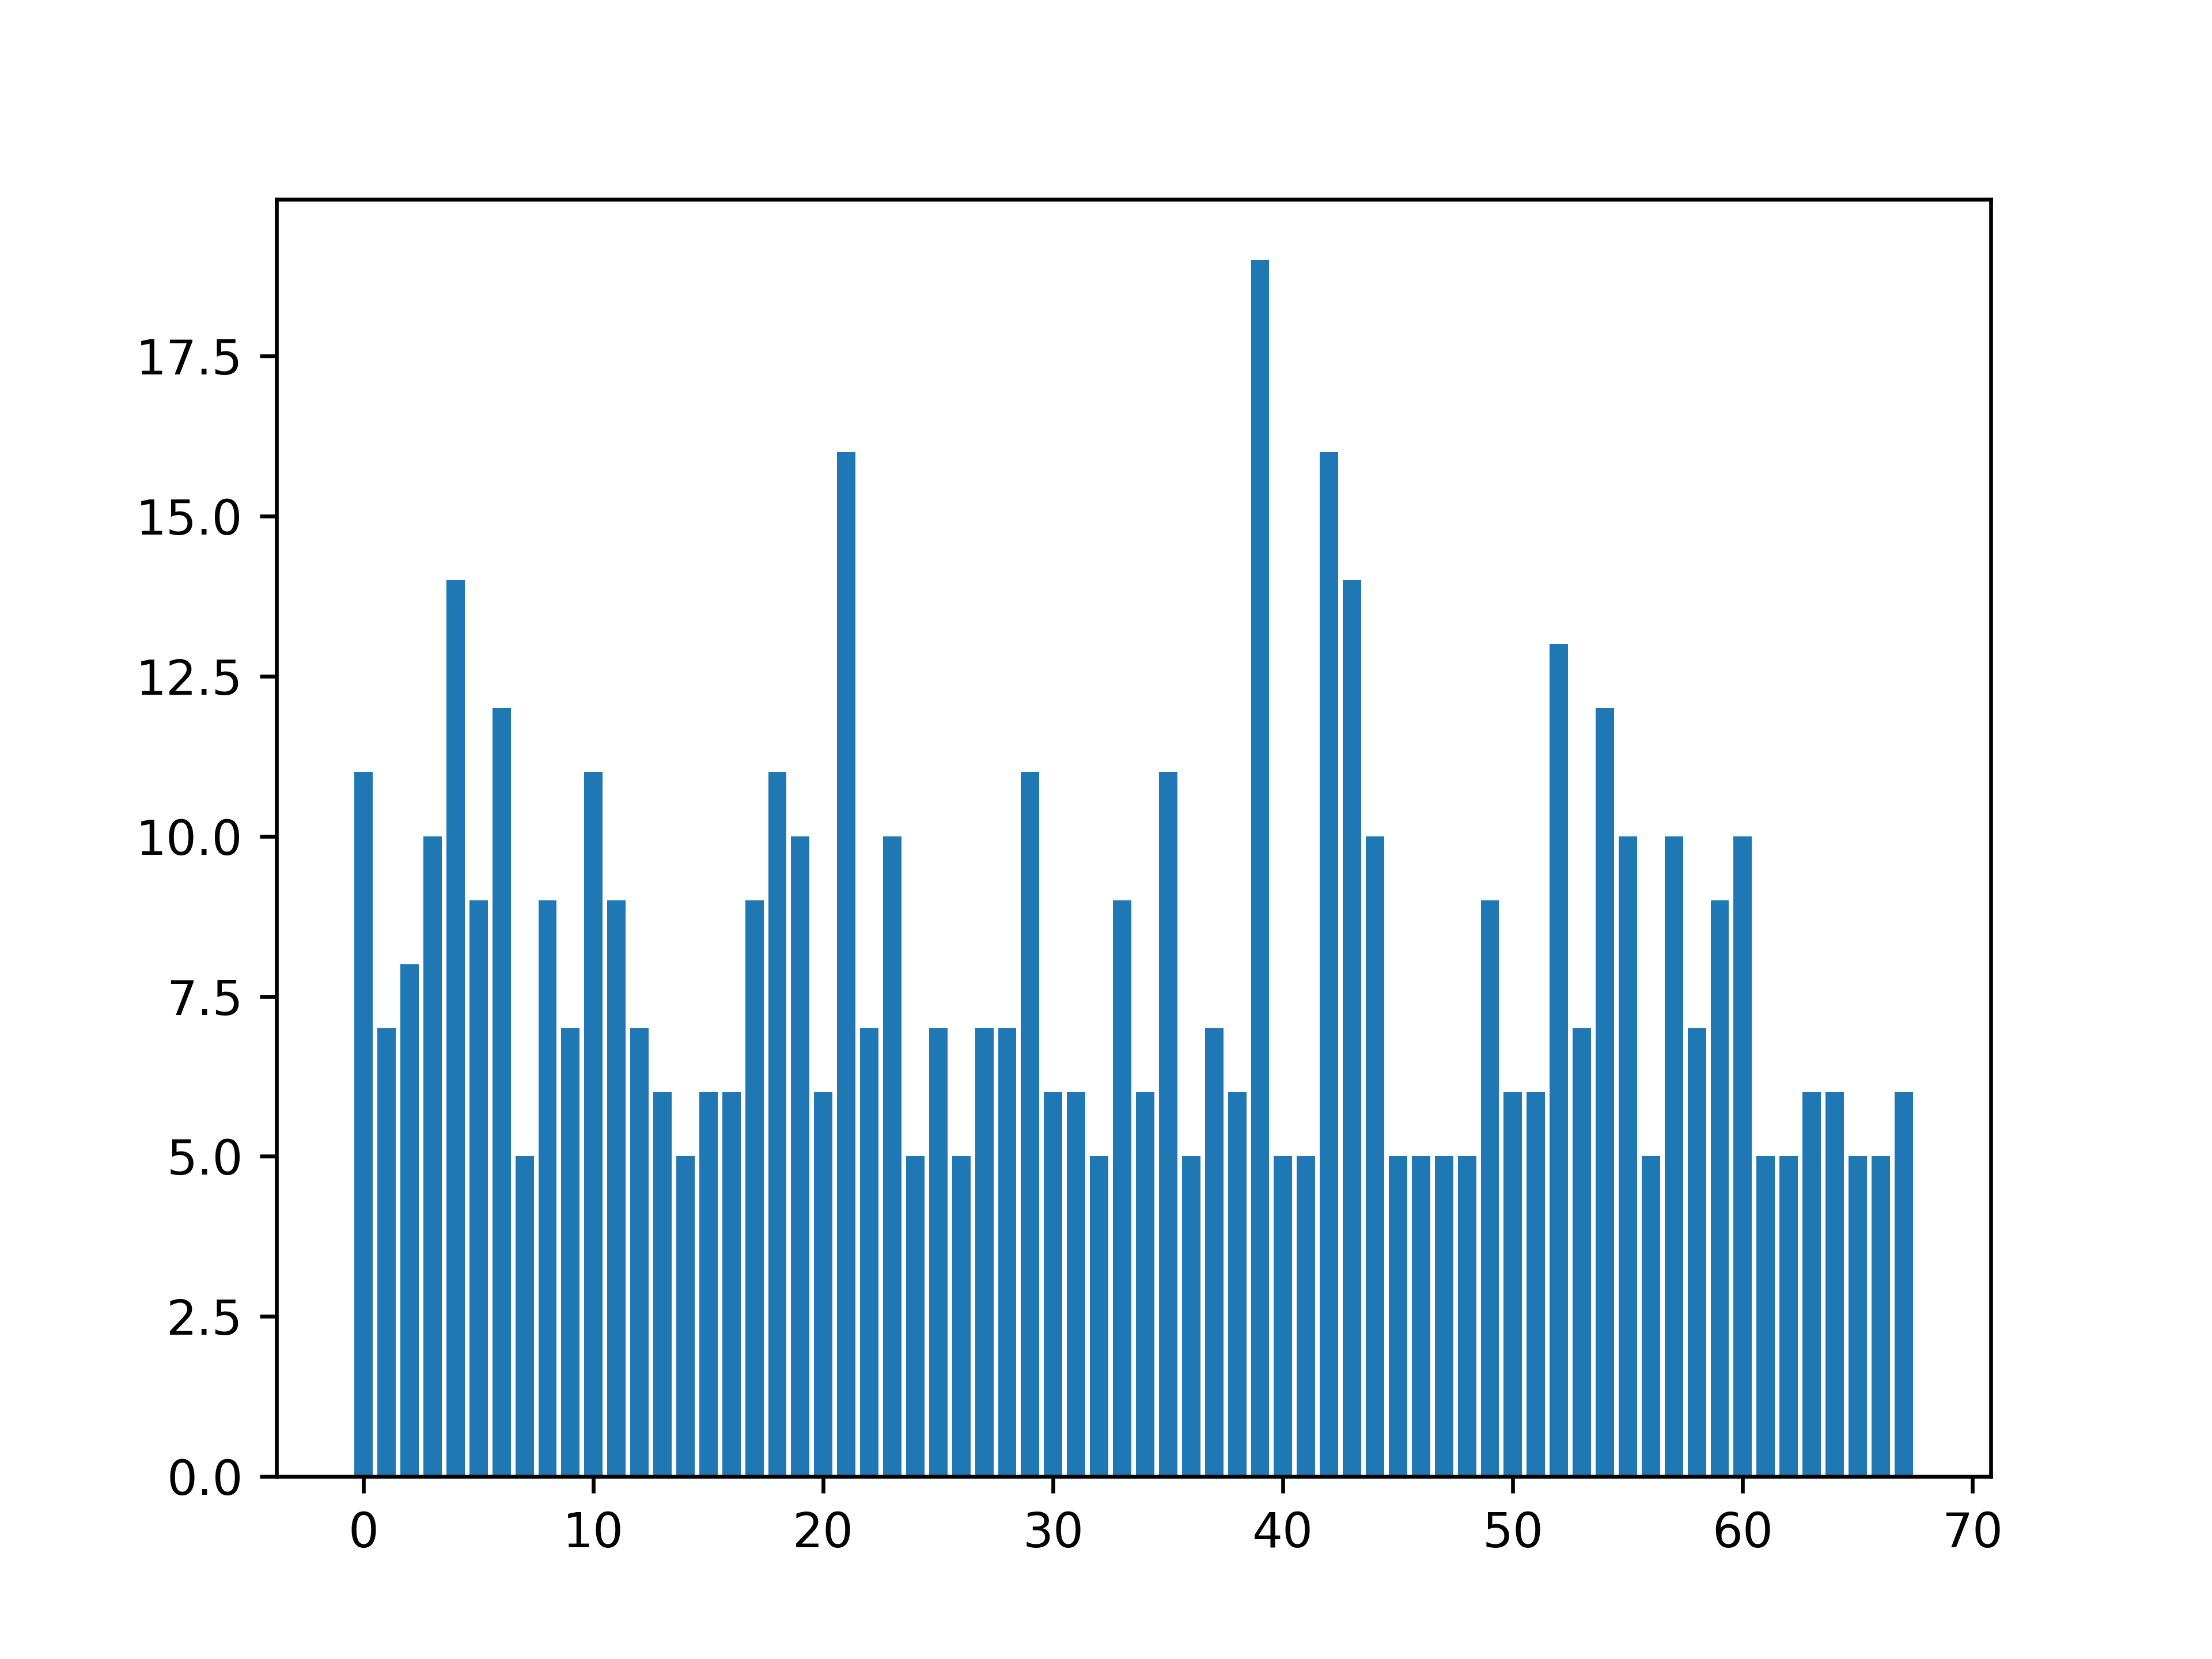
\includegraphics[width=0.75\textwidth]{cluster_distribution_species.png}
%    \caption{Size distribution of the \\ cluster of species.}
    \vspace{4ex}
  \end{minipage}%%
  \begin{minipage}[b]{0.5\linewidth}
    \centering
     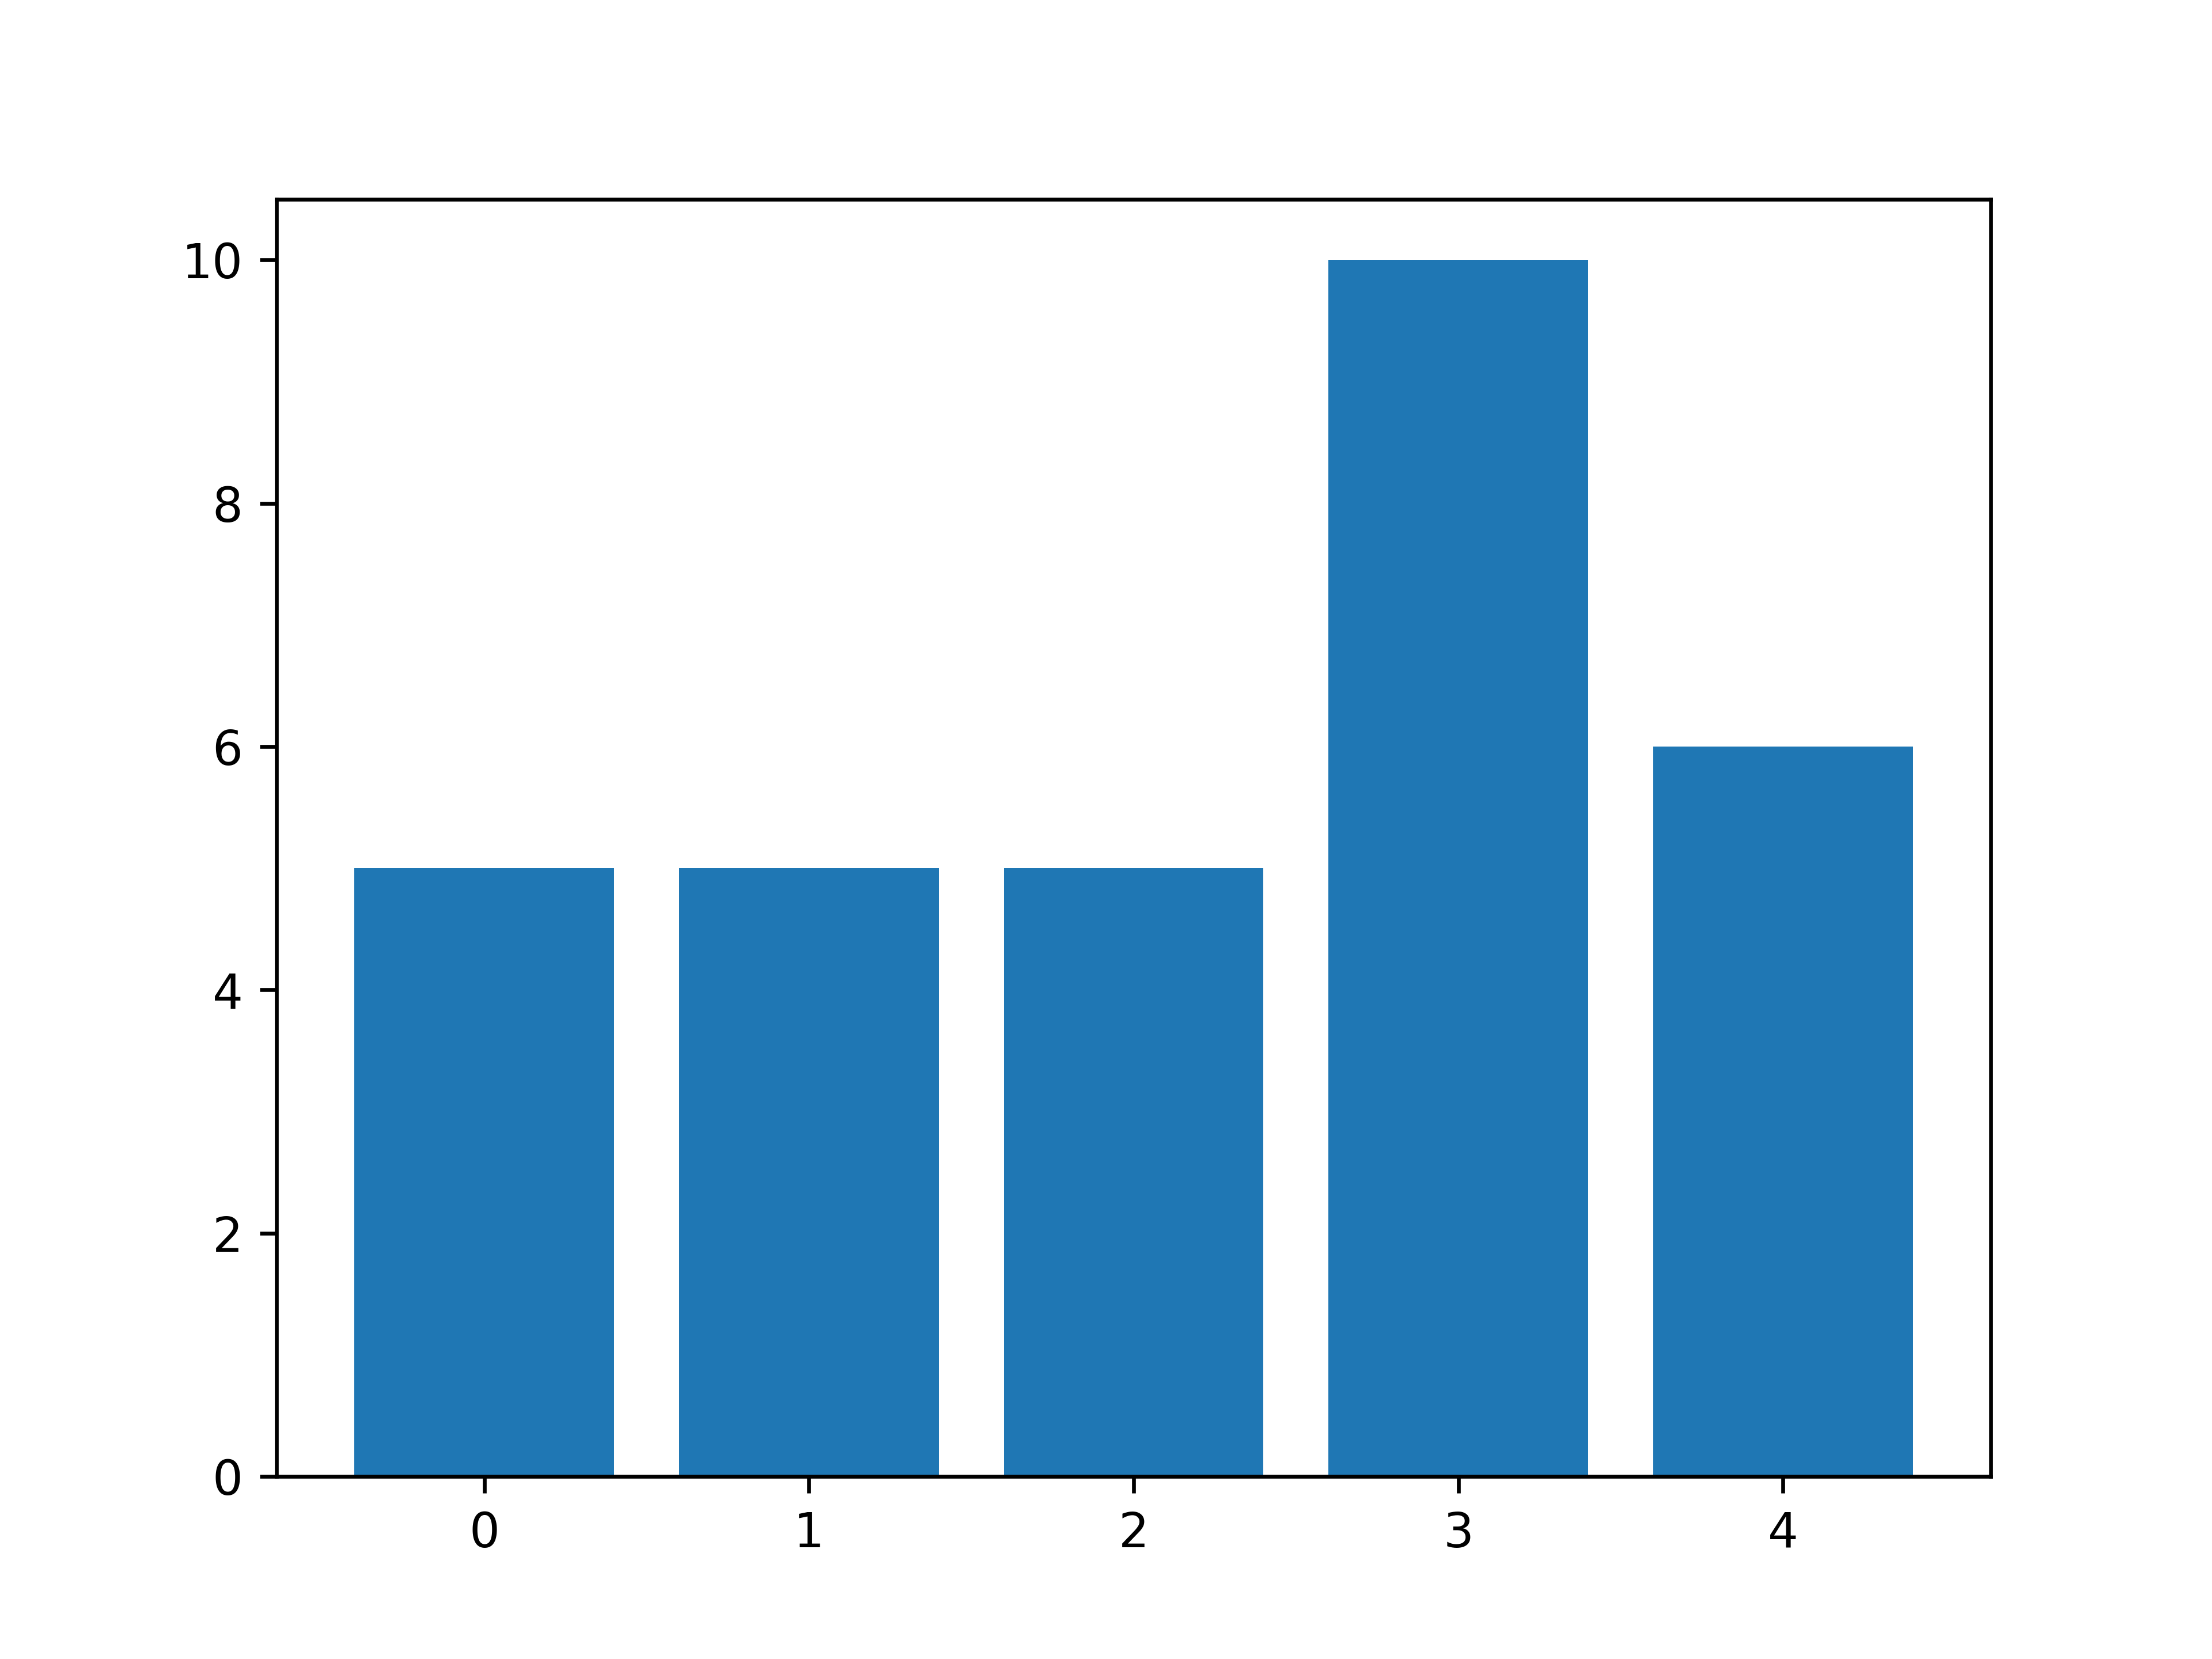
\includegraphics[width=0.75\textwidth]{cluster_distribution_region.png}
%    \caption{Size distribution of the \\ cluster of region.}
    \vspace{4ex}
  \end{minipage} 
%\caption{Cluster dimension.}
\caption{Size distribution of the cluster of species (left) and region (right).}
\label{fig:cluster_density}
\end{figure}

We now focus on analysing the taxonomic families of the species belonging to the five largest clusters. Out of the 18 Taxonomic Families, only 9 are present in the five largest clusters. This shows that some taxonomic families are more prominent to co-invade than others. In Table \ref{table:clusters_species} we reported the composition of the five largest clusters. If a taxonomic family is not found in a cluster, the entry is left empty. The plants family seems to have a significant relevance, it is present in all the clusters.  Birds and Insects seem to have the tendency to belong in the same clusters, meaning that they are likely to co-invade a region.

The dimension of the Taxonomic Families is non-homogeneous. As shown in Fig. \ref{fig:hist_tax_fam}, Vascular Plants and the Insects are the largest Taxonomic Families. This should be taken into account when analysing the composition of clusters: a species belonging to one of the most abundant families will have an higher probability of (indirectly) interacting with other species in the latent space. In fact, plants and insects are generally the largest components of the clusters we detected.

\begin{table}[H]
\centering
\begin{tabular}{|l|l|l|l|l|l|}
\hline
                & Cluster 4 & Cluster 21 & Cluster 39 & Cluster 42 & Cluster 43 \\ \hline
Algae           &           &            & 11 \%      &            &            \\ \hline
Birds           & 7 \%      & 6 \%       &            &            & 7 \%       \\ \hline
Crustaceans     & 7 \%      &            & 16 \%      & 6 \%       &            \\ \hline
Fishes          &           &            & 5 \%       & 6 \%       &            \\ \hline
Fungi           &           &            &            & 6 \%       &            \\ \hline
Insects         & 14 \%     & 12 \%      & 16 \%      &            & 36 \%      \\ \hline
Mammals         & 7 \%      &            &            &            &            \\ \hline
Reptiles        &           & 6 \%       &            &            &            \\ \hline
Vascular plants & 64 \%     & 75 \%      & 53 \%      & 81 \%      & 57 \%      \\ \hline
\end{tabular}
\caption{Species clusters composition.}
\label{table:clusters_species}
\end{table}


\section{Insights from the regions clusters}

The clusters for the regions in the latent space are also interesting. Applying the OPTICS clustering algorithm to the trajectories of the regions in the latent space detected $5$ clusters. They are reported in Table \ref{table:clusters_region}. For better visualization, the regions are reported respectively with different colors for the cluster they belong to in Fig. \ref{fig:worldmap_cluster}.  It's interesting to note how some clusters in the latent space are close in terms of distance such as the regions belonging to the clusters number 3 and 4. Regions that are geographically close are expected to be invaded by the same group of species. However, this effect does not apply to all regions. Cluster $1$, in particular, contains regions that are geographically not adjacent. This relation might be due to tight trade routes between these states.


\begin{table}[H]
\centering
\begin{tabular}{|l|l|l|l|l|}
\hline
Cluster 0 & Cluster 1                 & Cluster 2  & Cluster 3           & Cluster 4                \\ \hline
Russia    & Armenia                   & Lesotho    & Peru                & Iraq                     \\ \hline
Italy     & Chad                      & Mauritania & Andorra             & Nicaragua                \\ \hline
Canada    & Iran  & Gibraltar  & Belize              & Niger                    \\ \hline
Estonia   & Mongolia                  & Nepal      & Burkina Faso        & Vietnam                  \\ \hline
Slovakia  & Somalia                   & Suriname   & Libya               & Zambia                   \\ \hline
          &                           &            & Palestine & Central African Republic \\ \hline
          &                           &            & Senegal             &                          \\ \hline
          &                           &            & Tajikistan          &                          \\ \hline
          &                           &            & Gabon               &                          \\ \hline
          &                           &            & Congo               &                          \\ \hline
\end{tabular}
\caption{Region clusters composition.}
\label{table:clusters_region}
\end{table}

%TODO some regions are missing! fix it
\begin{figure}[ht]
    \centering
    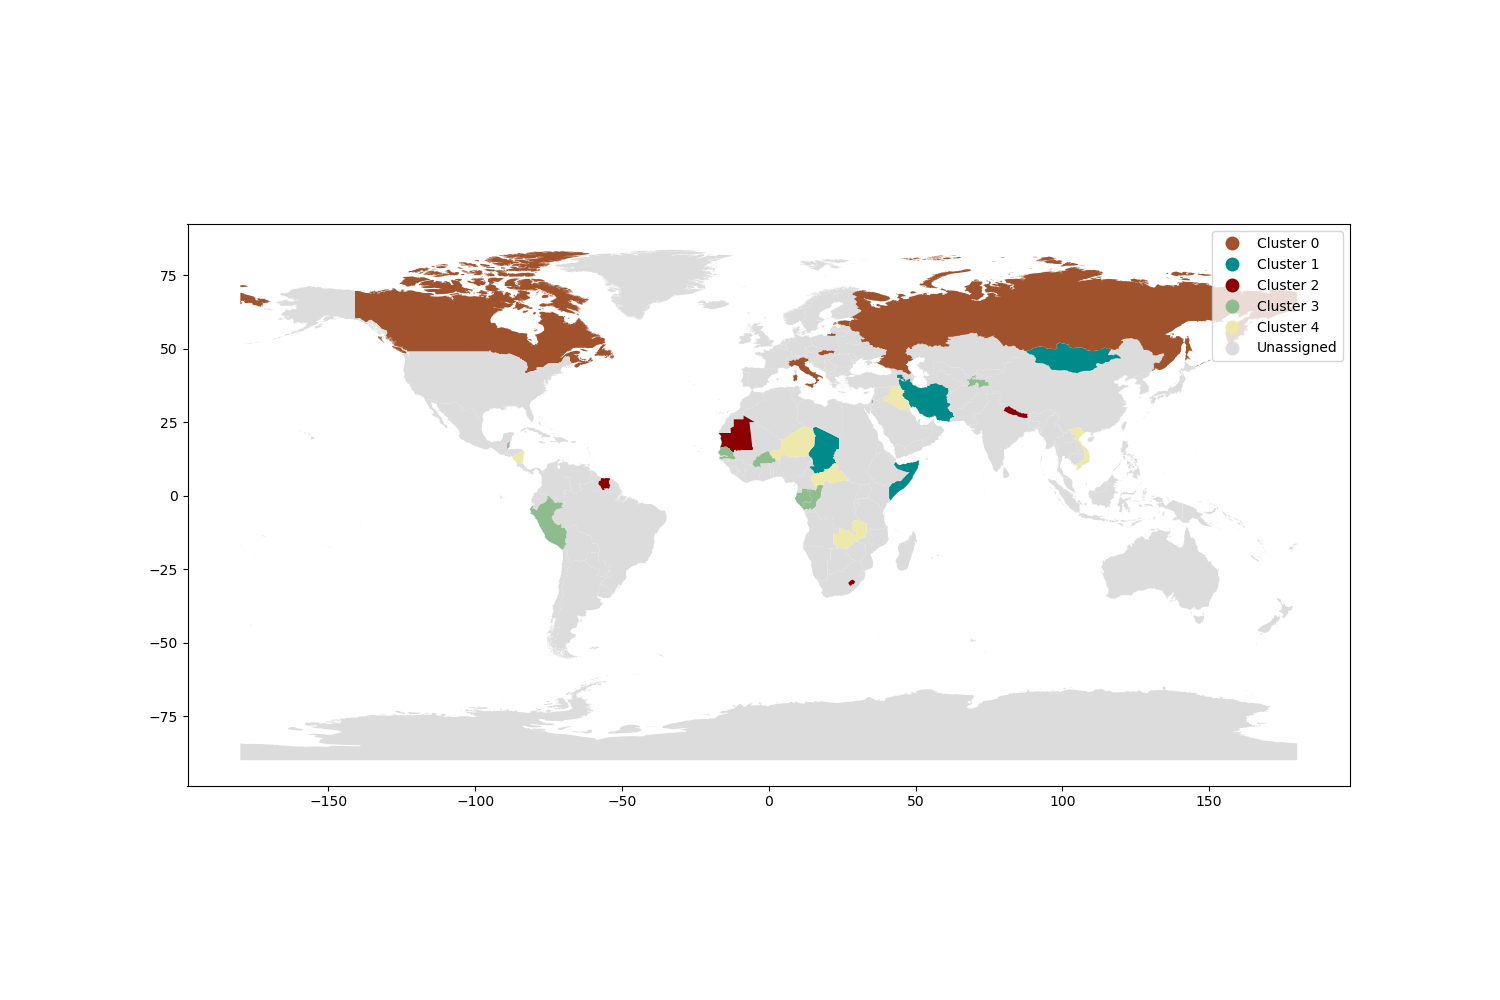
\includegraphics[width=0.85\textwidth]{region_geospatial_cluster.png}
    \caption{The five clusters of regions on the world map.}
    \label{fig:worldmap_cluster}
\end{figure}


%\section{Discussion}
%TODO write the conclusion of this chapter. Not sure what to say?


\chapter{Conclusion}

%1. Methodological contribution
The problem of alien species requires real action but without first understanding the in-depth drivers of invasion it's hard to come up with any action at all. In the last decades, relational event models have been successfully used to study the underneath drivers of dynamic social networks. Originally, relational event models were designed for small scale social networks. However, a traditional REM approach might not be always feasible due to the large size and complexity of a dataset and its high computationally cost.

In this thesis, we showed how to dispose of the actors of a relational event model in a 2-dimensional latent space and how to make inferences about it. Our inference approach combined many different tools such as the Expectation-Maximization algorithm, Kalman filters, and smoothers. Our method formulation can be applied to many different use cases and has many advantages over traditional statistical tools such as dimensionality reduction, a compact local configuration history of nodes, and large flexibility. Our study on the alien species co-invasion shows that the method is feasible for a real-world study. However, with the correct amount of modifications, our model can be applied to different problems and is not only limited to the study of a bipartite unidirectional graph as presented in this thesis. 

%2. Analysis done
We showed the applicability of our model by analyzing 15947 alien species invasions given by First Records Dataset. The analysis of the results of our model is based on studying clusters of trajectories in the latent space for both species and regions. We detected 67 clusters for the species and 5 for the regions in the latent space. Due to the high number of clusters found in the species, we focused on the 5 largest ones resulting in a non-exhaustive analysis. This approach is acceptable for a first analysis and to show the capabilities of our custom latent space REM, but, for an in-depth study of the co-invasion of species, this is not sufficient. A more exhaustive approach would have been to study the probability of, given a species, or a taxonomic family, finding another species inside all the clusters found in the analysis. 
 
%3. limitation: sigma choice is somehow arbitrary
Our approach requires the user to select the amount of noise $\Sigma$ that our model will use in the latent space process. A large $\Sigma$ will grant the model more dynamicity. In contrast, a small $\Sigma$ will make the model more conservative. The choice of this parameter is somehow arbitrary. A user might want to try different values of $\Sigma$ and analyze the dynamics of the latent space. Then, based on this feedback, update the value $\Sigma$ by either increasing or decreasing it. 

The First Records Dataset is currently the most comprehensive and largest dataset available for first-time records of alien species. However, it is a biased dataset towards regions such as Europe as a whole and taxonomic groups such as plants and insects. Furthermore, the information about the year of introduction of an alien species in a region is not precise and most of the time does not correspond to the year of actual introduction, which might have happened decades later. These biases and the unreliability of the dataset affected our results.

% Recap + conclusion
Concluding, we showed how a relational event model can be applied to a bipartite dynamic network and extended by including a latent space configuration of the nodes. We then presented to the reader a framework to analyze the results based on a clustering algorithm. The improvements and extension of already existing tools such as relational event models into more advanced and efficient methods capable of performing time-dependent analysis such as the study of alien species' first records will help ecologists to investigate this ecological phenomenon in-depth and to come up with real-world actions. 


%\nocite{*}

%\appendix %optional, use only if you have an appendix

%\chapter{e retarded material}
%\section{it is over\dots}
%\lipsum 
%
%\backmatter


%\chapter{Glossary} %optional

%\bibliographystyle{alpha}
%\bibliographystyle{dcu}
%\bibliographystyle{plainnat}
%\bibliography{biblio}

%\bibliographystyle{abbrvnat}
\bibliographystyle{plain} % We choose the "plain" reference style
\bibliography{biblio} % Entries are in the refs.bib file
%\cleardoublepage
%\theindex %optional, use only if you have an index, must use
	  %\makeindex in the preamble
%\lipsum

\end{document}
